% This is the Reed College LaTeX thesis template. Most of the work
% for the document class was done by Sam Noble (SN), as well as this
% template. Later comments etc. by Ben Salzberg (BTS). Additional
% restructuring and APA support by Jess Youngberg (JY).
% Your comments and suggestions are more than welcome; please email
% them to cus@reed.edu
%
% See http://web.reed.edu/cis/help/latex.html for help. There are a
% great bunch of help pages there, with notes on
% getting started, bibtex, etc. Go there and read it if you're not
% already familiar with LaTeX.
%
% Any line that starts with a percent symbol is a comment.
% They won't show up in the document, and are useful for notes
% to yourself and explaining commands.
% Commenting also removes a line from the document;
% very handy for troubleshooting problems. -BTS

% As far as I know, this follows the requirements laid out in
% the 2002-2003 Senior Handbook. Ask a librarian to check the
% document before binding. -SN

%%
%% Preamble
%%
% \documentclass{<something>} must begin each LaTeX document
\documentclass[12pt,twoside]{reedthesis}
% Packages are extensions to the basic LaTeX functions. Whatever you
% want to typeset, there is probably a package out there for it.
% Chemistry (chemtex), screenplays, you name it.
% Check out CTAN to see: http://www.ctan.org/
%%
\usepackage{graphicx,latexsym}
\usepackage{amsmath}
\usepackage{amssymb,amsthm}
\usepackage{longtable,booktabs,setspace}
\usepackage{chemarr} %% Useful for one reaction arrow, useless if you're not a chem major
\usepackage[hyphens]{url}
% Added by CII
\usepackage{hyperref}
\usepackage{lmodern}
\usepackage{float}
\floatplacement{figure}{H}
% End of CII addition
\usepackage{rotating}

% Next line commented out by CII
%%% \usepackage{natbib}
% Comment out the natbib line above and uncomment the following two lines to use the new
% biblatex-chicago style, for Chicago A. Also make some changes at the end where the
% bibliography is included.
%\usepackage{biblatex-chicago}
%\bibliography{thesis}


% Added by CII (Thanks, Hadley!)
% Use ref for internal links
\renewcommand{\hyperref}[2][???]{\autoref{#1}}
\def\chapterautorefname{Chapter}
\def\sectionautorefname{Section}
\def\subsectionautorefname{Subsection}
% End of CII addition

% Added by CII
\usepackage{caption}
\captionsetup{width=5in}
% End of CII addition

% \usepackage{times} % other fonts are available like times, bookman, charter, palatino

% Syntax highlighting #22
  \usepackage{color}
  \usepackage{fancyvrb}
  \newcommand{\VerbBar}{|}
  \newcommand{\VERB}{\Verb[commandchars=\\\{\}]}
  \DefineVerbatimEnvironment{Highlighting}{Verbatim}{commandchars=\\\{\}}
  % Add ',fontsize=\small' for more characters per line
  \usepackage{framed}
  \definecolor{shadecolor}{RGB}{248,248,248}
  \newenvironment{Shaded}{\begin{snugshade}}{\end{snugshade}}
  \newcommand{\KeywordTok}[1]{\textcolor[rgb]{0.13,0.29,0.53}{\textbf{#1}}}
  \newcommand{\DataTypeTok}[1]{\textcolor[rgb]{0.13,0.29,0.53}{#1}}
  \newcommand{\DecValTok}[1]{\textcolor[rgb]{0.00,0.00,0.81}{#1}}
  \newcommand{\BaseNTok}[1]{\textcolor[rgb]{0.00,0.00,0.81}{#1}}
  \newcommand{\FloatTok}[1]{\textcolor[rgb]{0.00,0.00,0.81}{#1}}
  \newcommand{\ConstantTok}[1]{\textcolor[rgb]{0.00,0.00,0.00}{#1}}
  \newcommand{\CharTok}[1]{\textcolor[rgb]{0.31,0.60,0.02}{#1}}
  \newcommand{\SpecialCharTok}[1]{\textcolor[rgb]{0.00,0.00,0.00}{#1}}
  \newcommand{\StringTok}[1]{\textcolor[rgb]{0.31,0.60,0.02}{#1}}
  \newcommand{\VerbatimStringTok}[1]{\textcolor[rgb]{0.31,0.60,0.02}{#1}}
  \newcommand{\SpecialStringTok}[1]{\textcolor[rgb]{0.31,0.60,0.02}{#1}}
  \newcommand{\ImportTok}[1]{#1}
  \newcommand{\CommentTok}[1]{\textcolor[rgb]{0.56,0.35,0.01}{\textit{#1}}}
  \newcommand{\DocumentationTok}[1]{\textcolor[rgb]{0.56,0.35,0.01}{\textbf{\textit{#1}}}}
  \newcommand{\AnnotationTok}[1]{\textcolor[rgb]{0.56,0.35,0.01}{\textbf{\textit{#1}}}}
  \newcommand{\CommentVarTok}[1]{\textcolor[rgb]{0.56,0.35,0.01}{\textbf{\textit{#1}}}}
  \newcommand{\OtherTok}[1]{\textcolor[rgb]{0.56,0.35,0.01}{#1}}
  \newcommand{\FunctionTok}[1]{\textcolor[rgb]{0.00,0.00,0.00}{#1}}
  \newcommand{\VariableTok}[1]{\textcolor[rgb]{0.00,0.00,0.00}{#1}}
  \newcommand{\ControlFlowTok}[1]{\textcolor[rgb]{0.13,0.29,0.53}{\textbf{#1}}}
  \newcommand{\OperatorTok}[1]{\textcolor[rgb]{0.81,0.36,0.00}{\textbf{#1}}}
  \newcommand{\BuiltInTok}[1]{#1}
  \newcommand{\ExtensionTok}[1]{#1}
  \newcommand{\PreprocessorTok}[1]{\textcolor[rgb]{0.56,0.35,0.01}{\textit{#1}}}
  \newcommand{\AttributeTok}[1]{\textcolor[rgb]{0.77,0.63,0.00}{#1}}
  \newcommand{\RegionMarkerTok}[1]{#1}
  \newcommand{\InformationTok}[1]{\textcolor[rgb]{0.56,0.35,0.01}{\textbf{\textit{#1}}}}
  \newcommand{\WarningTok}[1]{\textcolor[rgb]{0.56,0.35,0.01}{\textbf{\textit{#1}}}}
  \newcommand{\AlertTok}[1]{\textcolor[rgb]{0.94,0.16,0.16}{#1}}
  \newcommand{\ErrorTok}[1]{\textcolor[rgb]{0.64,0.00,0.00}{\textbf{#1}}}
  \newcommand{\NormalTok}[1]{#1}

% To pass between YAML and LaTeX the dollar signs are added by CII
\title{A dissertation}
\author{Jessica L. Burnett}
% The month and year that you submit your FINAL draft TO THE LIBRARY (May or December)
\date{2019}
\division{}
\advisor{Craig R. Allen}
\institution{University of Nebraska-Lincoln}
\degree{Doctor of Philosophy}
%If you have two advisors for some reason, you can use the following
% Uncommented out by CII
\altadvisor{Dirac Twidwell}
% End of CII addition

%%% Remember to use the correct department!
\department{School of Natural Resources}
% if you're writing a thesis in an interdisciplinary major,
% uncomment the line below and change the text as appropriate.
% check the Senior Handbook if unsure.
%\thedivisionof{The Established Interdisciplinary Committee for}
% if you want the approval page to say "Approved for the Committee",
% uncomment the next line
%\approvedforthe{Committee}

% Added by CII
%%% Copied from knitr
%% maxwidth is the original width if it's less than linewidth
%% otherwise use linewidth (to make sure the graphics do not exceed the margin)
\makeatletter
\def\maxwidth{ %
  \ifdim\Gin@nat@width>\linewidth
    \linewidth
  \else
    \Gin@nat@width
  \fi
}
\makeatother

\renewcommand{\contentsname}{Table of Contents}
% End of CII addition

\setlength{\parskip}{0pt}

% Added by CII

\providecommand{\tightlist}{%
  \setlength{\itemsep}{0pt}\setlength{\parskip}{0pt}}

\Acknowledgements{
Graduate school itself isn't hard, but the journey is. I have a lot of
people and institutions to thank for their emotional, intellectual,
financial, and other professional support. I wish to first highlight how
\textbf{great it was to be a graduate student at this university and in
the School of Natural Resources}. I have received tremendous support at
all levels of the university. Although I am not a fan of Nebraska's
climate, I highly recommend this school to prospective students. First,
I thank my supervisors, Craig Allen and Dirac Twidwell, for providing me
with this amazing opportunity and for supporting my growth as an
independent researcher. I thank my committee members, Craig Allen, David
Angeler, John De Long, Dirac Twidwell, and Drew Tyre for their support
and advisement, but especially for their comprehensive examination--I
found this process transformative. I especially thank Dirac for his
comprehensive exam questions--I never knew how much theory I didn't know
until I studied your list\ldots{} \textbf{Financial support}. This
research was funded by the U.S. Department of Defense's Strategic
Environmental Research and Development Program (project ID: RC-2510).
The University of Nebraska-Lincoln (UNL) has been highy supportive in my
doctoral studies and reserach. I am grateful for the generous of donors
to the University of Nebraska Foundation, which provided me with two
prestigious supplemental fellowships: Fling and Othmer. I also thank the
Nelson Family (Nelson Memorial Fellowship) and the Institute of
Agriculture and Natural Resources, who funded large portions of my
academic and research-related travel. I thank the School of Natural
Resources for their financial support in my conference travel. The U.S.
National Academy of Sciences generously funded part of my travel to the
International Institute for Applied Systems Analysis (IIASA). This
financial support provided me not only with invaluabe opportunities to
attend and present at national and international conferences and
workshops, conduct research abroad, and network--this funding alleviated
some financial pressures associated with graduate school which allowed a
more refined focus on my research. The opportunities and experiences
provided to me by these funding sources were amazing, thank you all.
\textbf{Emotional support}. I am one of the many graduate students
afflicted with mental health ``disorders'' which negatively impact my
quality of life, at times. I am first grafteful to one friend who
unknowingly destigmatized mental health, without which I may not have
sought treatment and diagnosis--thank you, Hannah. Since my diagnoses, I
have tried to encourage this destigmatization among graduate students in
our department. I thank felow students and faculty who have also been
outspoken regarding related issues (Jamilynn Polletto and Drew Tyre).
Finally, I thank Terry Thomas for her patience, support, and knowledge
as my general practitioner and mental health advocate.\\
I thank others for their various and probably unknowing contributions to
my professional development: David Angeler, Christie Bahlai, Hannah
Birge, Mary Bomberger Brown, John Carroll, Jenny Dauer, John DeLong,
Tarsha Eason, Brian Fath, Ahjond Garmestani, Chris Lepczyk, Frank La
Sorte, Chai Molina, Erica Stuber, Zac Warren, Lyndsie Wszola, Hao Ye,
Peter Zebrowski. I would like to especially thank some of the amazing
and brilliant \textbf{female scientists} in my life for their
encouragement: Jane Anderson, Hannah Birge, Mary Bomberger Brown, Tori
Donovan, Brittany Dueker, Allie Schiltmeyer, Katie Sieving, Erica
Stuber, and Lyndsie Wszola.
\begin{enumerate}
\def\labelenumi{\arabic{enumi}.}
\item
  \textbf{Federal employment}. One reason for coming to this program was
  specifically to study in a USGS Cooperative Research Unit, and to
  understand better life as a federal scientist. I thank Craig Allen and
  Kevin Pope for entertaining many hours of discussion (interrogation?)
  regarding federal employment.
\item
  \textbf{IIASA}. Studying at the International Institute for Applied
  Systems Analysis was an amazing opportunity. I thank Brian Fath and
  Elena Rovenskaya for their advisement, members of the Applied Systems
  Analysis research group for their feedback on my research, and to the
  postdocs and YSSPers.
\end{enumerate}
HEB, TD, CPR, DF, CRA, BF, ER, CAL, MPM, KES, FL, MBB,
\begin{enumerate}
\def\labelenumi{\arabic{enumi}.}
\tightlist
\item
  \textbf{Professional development}. AJT, KP, CRA, DT, MBB, JC,
\end{enumerate}
To my partner of eight years--Schultzie--thank you for everything. Just
kidding, thank you, Nat Price.
}

\Dedication{
Something snarky to mike moulton -- maybe a limerick
}

\Preface{
This is an example of a thesis setup to use the reed thesis document
class (for LaTeX) and the R bookdown package, in general.
}

\Abstract{
THis is my amazing abstract.
}

% End of CII addition
%%
%% End Preamble
%%
%
\begin{document}

% Everything below added by CII
  \maketitle

\frontmatter % this stuff will be roman-numbered
\pagestyle{empty} % this removes page numbers from the frontmatter
  \begin{acknowledgements}
    Graduate school itself isn't hard, but the journey is. I have a lot of
    people and institutions to thank for their emotional, intellectual,
    financial, and other professional support. I wish to first highlight how
    \textbf{great it was to be a graduate student at this university and in
    the School of Natural Resources}. I have received tremendous support at
    all levels of the university. Although I am not a fan of Nebraska's
    climate, I highly recommend this school to prospective students. First,
    I thank my supervisors, Craig Allen and Dirac Twidwell, for providing me
    with this amazing opportunity and for supporting my growth as an
    independent researcher. I thank my committee members, Craig Allen, David
    Angeler, John De Long, Dirac Twidwell, and Drew Tyre for their support
    and advisement, but especially for their comprehensive examination--I
    found this process transformative. I especially thank Dirac for his
    comprehensive exam questions--I never knew how much theory I didn't know
    until I studied your list\ldots{} \textbf{Financial support}. This
    research was funded by the U.S. Department of Defense's Strategic
    Environmental Research and Development Program (project ID: RC-2510).
    The University of Nebraska-Lincoln (UNL) has been highy supportive in my
    doctoral studies and reserach. I am grateful for the generous of donors
    to the University of Nebraska Foundation, which provided me with two
    prestigious supplemental fellowships: Fling and Othmer. I also thank the
    Nelson Family (Nelson Memorial Fellowship) and the Institute of
    Agriculture and Natural Resources, who funded large portions of my
    academic and research-related travel. I thank the School of Natural
    Resources for their financial support in my conference travel. The U.S.
    National Academy of Sciences generously funded part of my travel to the
    International Institute for Applied Systems Analysis (IIASA). This
    financial support provided me not only with invaluabe opportunities to
    attend and present at national and international conferences and
    workshops, conduct research abroad, and network--this funding alleviated
    some financial pressures associated with graduate school which allowed a
    more refined focus on my research. The opportunities and experiences
    provided to me by these funding sources were amazing, thank you all.
    \textbf{Emotional support}. I am one of the many graduate students
    afflicted with mental health ``disorders'' which negatively impact my
    quality of life, at times. I am first grafteful to one friend who
    unknowingly destigmatized mental health, without which I may not have
    sought treatment and diagnosis--thank you, Hannah. Since my diagnoses, I
    have tried to encourage this destigmatization among graduate students in
    our department. I thank felow students and faculty who have also been
    outspoken regarding related issues (Jamilynn Polletto and Drew Tyre).
    Finally, I thank Terry Thomas for her patience, support, and knowledge
    as my general practitioner and mental health advocate.\\
    I thank others for their various and probably unknowing contributions to
    my professional development: David Angeler, Christie Bahlai, Hannah
    Birge, Mary Bomberger Brown, John Carroll, Jenny Dauer, John DeLong,
    Tarsha Eason, Brian Fath, Ahjond Garmestani, Chris Lepczyk, Frank La
    Sorte, Chai Molina, Erica Stuber, Zac Warren, Lyndsie Wszola, Hao Ye,
    Peter Zebrowski. I would like to especially thank some of the amazing
    and brilliant \textbf{female scientists} in my life for their
    encouragement: Jane Anderson, Hannah Birge, Mary Bomberger Brown, Tori
    Donovan, Brittany Dueker, Allie Schiltmeyer, Katie Sieving, Erica
    Stuber, and Lyndsie Wszola.
    \begin{enumerate}
    \def\labelenumi{\arabic{enumi}.}
    \item
      \textbf{Federal employment}. One reason for coming to this program was
      specifically to study in a USGS Cooperative Research Unit, and to
      understand better life as a federal scientist. I thank Craig Allen and
      Kevin Pope for entertaining many hours of discussion (interrogation?)
      regarding federal employment.
    \item
      \textbf{IIASA}. Studying at the International Institute for Applied
      Systems Analysis was an amazing opportunity. I thank Brian Fath and
      Elena Rovenskaya for their advisement, members of the Applied Systems
      Analysis research group for their feedback on my research, and to the
      postdocs and YSSPers.
    \end{enumerate}
    HEB, TD, CPR, DF, CRA, BF, ER, CAL, MPM, KES, FL, MBB,
    \begin{enumerate}
    \def\labelenumi{\arabic{enumi}.}
    \tightlist
    \item
      \textbf{Professional development}. AJT, KP, CRA, DT, MBB, JC,
    \end{enumerate}
    To my partner of eight years--Schultzie--thank you for everything. Just
    kidding, thank you, Nat Price.
  \end{acknowledgements}
  \begin{preface}
    This is an example of a thesis setup to use the reed thesis document
    class (for LaTeX) and the R bookdown package, in general.
  \end{preface}
  \hypersetup{linkcolor=black}
  \setcounter{tocdepth}{2}
  \tableofcontents

  \listoftables

  \listoffigures
  \begin{abstract}
    THis is my amazing abstract.
  \end{abstract}
  \begin{dedication}
    Something snarky to mike moulton -- maybe a limerick
  \end{dedication}
\mainmatter % here the regular arabic numbering starts
\pagestyle{fancyplain} % turns page numbering back on

\hypertarget{section}{\chapter*{}\label{section}}
\addcontentsline{toc}{chapter}{}

\chapter*{Preliminary Content}\label{preliminary-content}
\addcontentsline{toc}{chapter}{Preliminary Content}

Paste from index.rmd if knitting to git or html

\section*{Acknowledgements}\label{acknowledgements}
\addcontentsline{toc}{section}{Acknowledgements}

Paste from index.rmd if knitting to git or html

\section*{Preface}\label{preface}
\addcontentsline{toc}{section}{Preface}

Paste from index.rmd if knitting to git or html

\section*{Dedication}\label{dedication}
\addcontentsline{toc}{section}{Dedication}

Paste from index.rmd if knitting to git or html

THis is my amazing abstract.

\chapter{Introduction}\label{intro-chapter}

\section{Background}\label{background}

Abrupt changes in the environment - On abrupt changes in the environment
1. A few examples of abrupt changes that are highly referenced.\\
1. Why does it matter that we can detect?? 2. A few examples of the
methds that have been used ot identifythese shifts - histortically -
real-time - predictive 3. PRoblems with the methods in - aplpication -
difficult to apply - to interpret - theory - lackthereof 4. Descrive the
attempts to identify regime shifts - the most solid theoretical concept
in the field of regime shifts is the concept of \emph{critical slowing
down}

\section{Goal of the dissertation}\label{goal-of-the-dissertation}
\begin{enumerate}
\def\labelenumi{\arabic{enumi}.}
\tightlist
\item
  The goal of the works described herein is to evaluate methods proposed
  as indicators fo regime shift in \textbf{ecological communities}.\\
\item
  Propose simple, alternative methods to multispecies
\end{enumerate}
\begin{Shaded}
\begin{Highlighting}[]
\CommentTok{# Create a table of definitions }
  \CommentTok{# A box would be nice - if I have the time}
\NormalTok{defs_tbl <-}\StringTok{ }\KeywordTok{rbind}\NormalTok{(}
        \KeywordTok{c}\NormalTok{(}\StringTok{"Regime shift"}\NormalTok{, }\StringTok{"Vaguely defined as the change in the structure or functioning of a system."}\NormalTok{ , }\StringTok{'ref'}\NormalTok{), }
        \KeywordTok{c}\NormalTok{(}\StringTok{"Regine"}\NormalTok{,}\StringTok{"def"}\NormalTok{, }\StringTok{'ref'}\NormalTok{), }
        \KeywordTok{c}\NormalTok{(}\StringTok{"term"}\NormalTok{,}\StringTok{"def"}\NormalTok{, }\StringTok{'ref'}\NormalTok{), }
        \KeywordTok{c}\NormalTok{(}\StringTok{"term"}\NormalTok{,}\StringTok{"def"}\NormalTok{, }\StringTok{'ref'}\NormalTok{), }
        \KeywordTok{c}\NormalTok{(}\StringTok{"term"}\NormalTok{,}\StringTok{"def"}\NormalTok{, }\StringTok{'ref'}\NormalTok{), }
        \KeywordTok{c}\NormalTok{(}\StringTok{"term"}\NormalTok{,}\StringTok{"def"}\NormalTok{, }\StringTok{'ref'}\NormalTok{), }
        \KeywordTok{c}\NormalTok{(}\StringTok{"term"}\NormalTok{,}\StringTok{"def"}\NormalTok{, }\StringTok{'ref'}\NormalTok{), }
        \KeywordTok{c}\NormalTok{(}\StringTok{"term"}\NormalTok{,}\StringTok{"def"}\NormalTok{, }\StringTok{'ref'}\NormalTok{), }
        \KeywordTok{c}\NormalTok{(}\StringTok{"term"}\NormalTok{,}\StringTok{"def"}\NormalTok{, }\StringTok{'ref'}\NormalTok{)}
\NormalTok{        ) }\OperatorTok
\StringTok{  }\KeywordTok{data.frame}\NormalTok{() }\OperatorTok\StringTok{ }
\StringTok{  `}\DataTypeTok{colnames<-}\StringTok{`}\NormalTok{( }\KeywordTok{c}\NormalTok{(}\StringTok{"Regime shift"}\NormalTok{, }\StringTok{"definitions"}\NormalTok{, }\StringTok{"recomended source(s)"}\NormalTok{))}


\NormalTok{knitr}\OperatorTok{::}\KeywordTok{kable}\NormalTok{(defs_tbl, }\StringTok{"latex"}\NormalTok{, }\DataTypeTok{booktabs =}\NormalTok{ T,}
             \DataTypeTok{caption =} \StringTok{"Definitions of terms related to regime shifts appearing throughout this work. Terms are higlighted in bold in the following section only."}\NormalTok{) }\OperatorTok
\StringTok{  }\NormalTok{kableExtra}\OperatorTok{::}\KeywordTok{kable_styling}\NormalTok{(}\DataTypeTok{full_width =}\NormalTok{ F) }\OperatorTok
\StringTok{  }\NormalTok{kableExtra}\OperatorTok{::}\KeywordTok{column_spec}\NormalTok{(}\DecValTok{1}\NormalTok{, }\DataTypeTok{bold =}\NormalTok{ T, }\DataTypeTok{color =} \StringTok{"black"}\NormalTok{) }\OperatorTok\StringTok{ }\CommentTok{# adjsts column width to provide flexibility for text columns}
\StringTok{  }\NormalTok{kableExtra}\OperatorTok{::}\KeywordTok{column_spec}\NormalTok{(}\DecValTok{2}\NormalTok{, }\DataTypeTok{width =} \StringTok{"50em"}\NormalTok{) }\OperatorTok\StringTok{ }
\StringTok{  }\NormalTok{kableExtra}\OperatorTok{::}\KeywordTok{column_spec}\NormalTok{(}\DecValTok{3}\NormalTok{, }\DataTypeTok{width =} \StringTok{"30em"}\NormalTok{, }\DataTypeTok{color =} \StringTok{"grey"}\NormalTok{) }
\end{Highlighting}
\end{Shaded}
\begin{table}

\caption{(\#tab:tab:defs_tbl)Definitions of terms related to regime shifts appearing throughout this work. Terms are higlighted in bold in the following section only.}
\centering
\begin{tabular}[t]{>{\bfseries\leavevmode\color{black}}l>{\raggedright\arraybackslash}p{50em}>{\raggedright\arraybackslash\leavevmode\color{grey}}p{30em}}
\toprule
Regime shift & definitions & recomended source(s)\\
\midrule
Regime shift & Vaguely defined as the change in the structure or functioning of a system. & ref\\
Regine & def & ref\\
term & def & ref\\
term & def & ref\\
term & def & ref\\
\addlinespace
term & def & ref\\
term & def & ref\\
term & def & ref\\
term & def & ref\\
\bottomrule
\end{tabular}
\end{table}
Here is my reference to a table (\#tab:defs\_tbl)

\subsection{On critical slowing down}\label{on-critical-slowing-down}

\textbf{Critical slowing down} is the most solid theoretical concept in
the study of \textbf{ecological regime shifts} and is a more precise
variant of \textbf{Pimm's resilience} (c.f. \textbf{Hollings
resilience}). The theory is such that the \textbf{recovery rate}, or the
time it takes to return to a \textbf{stable} point, decreases as it
nears its \textbf{tipping point}.

``the recovery rate should decrease. It occurs because a system's
internal stabilizing forces become weaker near the point where they
break and the system moves into a new regime. Thus critical slowing down
is posited to exist at phase transitions, such as ecosystem collapse. A
system is stable when it is in a deep basin of attraction corresponding
to many strong negative feedback loops acting on it. In such a case
small perturbations do not have long-term consequences. As a system
degrades these negative feedback loops become broken and thus the
steepness of the basin of attraction becomes lower. Its resilience
becomes decreased bring the system close to a critical transition. This
means that the same perturbation that may not flip the system will
though likely take longer to dissipate. Thus it will take longer for the
system to return to its point of equilibrium when close to a tipping
point. The simplest way to measure the approach to a potential tipping
point then would be to directly measure the recovery rate at which the
system returns back to its initial equilibrium state following a
perturbation. In cases where the system is close to a tipping point, the
recovery rate should decrease -- slow down. As such critical slowing
down offers some potential to probe the dynamics of a system in order to
assess its resilience and the risk of an upcoming regime shift. ``We
have all these complex systems like the brain, the climate, ecosystems,
the financial market, that are really difficult to understand, and we
will probably never fully understand them. So it's really kind of a
small miracle that across these very different systems, we could find
these universal indicators of how close they are to a threshold'' --
Marten Scheffer''"

``I think the most solid theoretical concept in this field is
the''critical slowing down" which typically manifests itself as
increased variance or autocorrelation at a critical transition. Much has
been written about this, especially by Maarten Sceffer, Stephen
Carpenter et al.
(e.g.~\url{https://www.annualreviews.org/doi/abs/10.1146/annurev-ecolsys-112414-054242})
Common to all methods derived from this theoretically sound concept, is
that they need quite a lot of data - typically more than you would
usually have in ecological time series, at least. "

For multispecies data you will typically need to reduce dimensionality
before you can proceed, for example by some sort of ordination. The
vegan package for R is typically the starting point for this. I can help
you a bit further on the way if you are not familiar with this if you
want to, but then I would need to know a bit more about your data.

\subsection{Types fo regime shifts}\label{types-fo-regime-shifts}

There are different types fo regime shifts, and \textbf{why those
differences matter}
\begin{itemize}
\tightlist
\item
  only ``regime shifts'' that are also ``critical transitions'' should
  show ``critical slowing down''
  \begin{itemize}
  \tightlist
  \item
    so that's an important \emph{technical distinction} if you're trying
    to use \emph{``early warning signals''}.\\
  \end{itemize}
\item
  There are mutiple types og \textbf{critical transitions}
  \begin{itemize}
  \tightlist
  \item
    these results in very different changes in time series\\
  \item
    in some contexts, this doesn't really matter
  \end{itemize}
\end{itemize}
\section{Brandolini's principle}\label{brandolinis-principle}

TWo major sources of problems? 1. Defining a regime shift\\
2. Methods have not proven useful for application beyond single-species
systems and systems about which causal drivers can just be monitored.
\begin{itemize}
\tightlist
\item
  Current state of regime shift theory
\item
  Why it is important to diagnose/detect abrupt changes at the system
  level
\item
  Current methods are not being employed by ecological management.
  \begin{itemize}
  \tightlist
  \item
    Why are applications largely restricted to theoretical research?
  \item
    Why are the applications to empirical data largely restricted to the
    research community?
  \item
    Is this an artefact of how long it takes for applied ecologists and
    ecological management to adopt new data anlysis techniques?
  \end{itemize}
\end{itemize}
\section{Importance of this thesis}\label{importance-of-this-thesis}
\begin{itemize}
\tightlist
\item
  Identifying methods for multiple species data
\item
  Highlighting the methods that may or may not be useful to the causal
  quantitative ecologist
\end{itemize}
\chapter{Quantitative indicators of abrupt ecological
change}\label{indicators-chapter}

\section{Introduction}\label{introduction}

Regime shifts can be defined as changes in either the structure or
underlying functioning of a system. Identifying historic ecolgoical
regime changes has been achieved using post-hoc analyitcal approaches,
and many have been tested and verified in multiple systems. Methods for
reliably forecasting and predicting these changes are less common.
Although numerous quantitative methods exist for detecting ecological
regime shifts, new methods are proposed for achieving this aim ata XXX
rate (\emph{insert figure of number of papers per year with new
methods}). These methods have proven useful in detecting shifts in
atmospheric and fisheries catch data, and in systems that are
well-described by a few state variables, or can be modelled reliably
with matheamtical equations. Because ecological comunities are more
complex than, say, a simple Lotka-Volterra predator prey system, the set
of reliable regime shift detection methods narrows.

Ecological and social-ecolgical systems havemany unpredictable and
variably interacting components. Systems analyses, including Dynamic
Bayesian Networks, network models, and food webs are designed to handle
these complexities, yet obtaining enough information to feed these
models seems less feasible in ecosystem research and management. A
survey of the methods available for detecting ecological regime shifts
in high dimensional data is timely. Recent reviews of regime shift
indicators (Andersen et al, the others) are outdated, are not
comprehensive (include only a subset of the available RSDMs), and do not
provide recommendations for which events, systems, or data
characterstics are appropriate for these methods.

Some RSDMs are proposed for and are subsequently applied to data having
specific characteristics, while others are proposed to be useful in
multiple systems and on data of varying characterstics (e.g., Karunithi
et al; Mayer 2007; Eason). This review provides a summary of the
available methods and evaluates the appropriateness of these methods to
data of varying character, quality, and quantity.

This paper aims to identify, describe, and critique quantitative RSDMs
that have been used or proposed to detect regime shifts in ecological
data. We discuss the relevant characteristics of the data/information
that are required for each method, and how these characterstics may help
or hinder the ecologists' interpretation of the analytical results. We
pay special attention to the RSDMs that are most appropriate for
analysis of high dimensional and noisy ecological data.

\section{Methods}\label{methods}

\subsection{Identifying papers/RSDMs in the
literature}\label{identifying-papersrsdms-in-the-literature}
\begin{enumerate}
\def\labelenumi{\arabic{enumi}.}
\tightlist
\item
  We conducted a systematic review using the software Publish or Perish
  to identify unique statistical and numerical methods that have been
  used to identify ecological regime shifts. We used the following
  databases to identify scholarly works that introduce and/or explain
  methods for identfying regime shifts:
  \begin{enumerate}
  \def\labelenumii{\roman{enumii}.}
  \tightlist
  \item
    **Database searches*
    \begin{enumerate}
    \def\labelenumiii{\alph{enumiii}.}
    \tightlist
    \item
      Boolean (+ = asterisk in the database search)\\
      i. WOS:\\
      ii. SCOPUS: ( TITLE-ABS-KEY ( ( approach OR analysis OR metric OR
      method\^{} ) AND ( detect\^{} OR predict\^{} ) ) AND TITLE-ABS-KEY
      ( \{regime shift\} OR \{regime change\} OR \{abrupt change\} ) )
      \textbf{1,473} (where \^{}== ** in Scopus)
    \end{enumerate}
  \item
    \textbf{Opportunistic papers}
    \begin{enumerate}
    \def\labelenumiii{\alph{enumiii}.}
    \tightlist
    \item
      We used expert opinion (authors JLB, etc.) to identify any missing
      RSDMs that were not detected in our formal database searches. (i
      am making this next part up--need to double check once i have
      results)--\textgreater{}These papers are are typically found in
      the grey literature, or are published in journals not obvious to
      the general ecologist (e.g., name an obscure journal here).\\
    \item
      Justification for our database searches containing some of these
      methods which are known/obvious to the author(s).
    \end{enumerate}
  \end{enumerate}
\item
  Procedures for filtering the papers.
  \begin{enumerate}
  \def\labelenumii{\roman{enumii}.}
  \tightlist
  \item
    We removed duplicate titles (from the merging of Scopus and WOS),
    which resulted in **\_\_\_** unique scholarly works.\\
  \item
    We read the abstracts of each paper to determine the following:
    \begin{enumerate}
    \def\labelenumiii{\alph{enumiii}.}
    \tightlist
    \item
      Was this a new method being proposed or used? (if yes, proceed to
      ii.))\\
    \item
      Was this just a case study or another application of a previously
      published method? (if yes, note the method(s) used and identify
      original method(s) source)\\
    \item
      If this paper was an application of a method, we noted the method,
      and identified the orignal source for the method (if possible)\\
    \end{enumerate}
  \item
    Identify characteristics of the method
    \begin{enumerate}
    \def\labelenumiii{\alph{enumiii}.}
    \setcounter{enumiii}{2}
    \tightlist
    \item
      It is model-based?\\
    \item
      Does it require a mathematical model?
    \item
      Does it require \emph{a priori} knowledge of the regime shift
    \item
      Does it forecast or provide predicitons?
    \item
      Assumptions required (e.g., discontinuity, step functions,
      normality of response vars)
    \end{enumerate}
  \item
    Identify requirements for the data input
    \begin{enumerate}
    \def\labelenumiii{\alph{enumiii}.}
    \tightlist
    \item
      Require equal spacing b/w observations?
    \item
      Minimum \# data points required to use?
    \item
      Minimum \# of state variables required?
    \end{enumerate}
  \item
    Identify the characteristics of the data USED to demonstrate the
    method
    \begin{enumerate}
    \def\labelenumiii{\alph{enumiii}.}
    \tightlist
    \item
      Spatial resolution and extent
    \item
      Temporal resolution and extent
    \item
      Number of state variables
    \item
      System type
    \item
      Whole-system vs.~selected variables?
    \end{enumerate}
    \begin{enumerate}
    \def\labelenumiii{\roman{enumiii}.}
    \setcounter{enumiii}{1}
    \tightlist
    \item
      Experimental system or observational/passive
    \end{enumerate}
  \end{enumerate}
\item
  Note the number of times the paper has been cited
\end{enumerate}
\section{Results}\label{results}

We identified **\_\_\_** number of quantiattive anlaytical approaches to
identifying regime shifts and abrupt changes in data.

\subsection{Potential figures}\label{potential-figures}
\begin{enumerate}
\def\labelenumi{\arabic{enumi}.}
\tightlist
\item
  X = year Y = number of publications for \emph{new} RSDMs in the
  ecol/env literature
\item
  X = year Y = \# pubs for new RSDM appropriate for multidimensional
  systems
\end{enumerate}
\subsection{Potential tables}\label{potential-tables}
\begin{longtable}[t]{lllll}
\caption{\label{tab:characteristicsResults}Data structure and analytical procedures characteristics fo the selected studies.}\\
\toprule
Authors & Year of Publication & Dimensionality of data & Longitudinality of data & Method applied\\
\bottomrule
\end{longtable}
\section{Discussion}\label{discussion}
\begin{enumerate}
\def\labelenumi{\arabic{enumi}.}
\tightlist
\item
  Major findings of the review.
\item
  What major assumptions are we currently making about the data and the
  system that we need to know more about moving forward? i.e., where are
  the gaps in knowledge?
\item
  How has or how can we take advantage of unstructured or
  semi-structured data to ID regime shifts?
\item
  How can or should we adapt our monitoring schemes to better suit these
  (or at least the seemingly helpful) analyses?
\item
  What about identifying the drivers behind the shifts?
\item
  Which methods posit they can identify the, or potential, drivers of
  the state changes? Which have shown it?
\end{enumerate}
Potential text: 1. Climate change is expected to induce an increase in
both the intensity and frequency of rapid ecological change or
disturbance, impacting social systems, potentially to the detriment of
human communities most vulnerable. Identifying and forecasting these
changes is critical for community and ecological planning, management,
and disaster mitigation.
\begin{enumerate}
\def\labelenumi{\arabic{enumi}.}
\item
  Because ecological and social systems are tightly coupled, we have
  used indicators in the environment and in wildlife communities to
  identify change and potential changes that may impact our social
  communities.
\item
  Many regime shift analytical papers suggest that, using multiple
  quantitative methods to provide for evidence for a regiem shift in a
  specific data set is necessary or is acceptable. Although this
  proposition is valid, comparing results within a single system using
  multiple methods has often yielded varying results. Managing systems
  using quantitative methods that yield different results may yield
  improper management techniques and objectives.
\end{enumerate}
\chapter{A guide to Fisher Information for Ecologists}\label{fiGuide}

\section{Abstract}\label{abstract}

Ecological regime shifts are increasingly prevalent in the Anthropocene.
The number of methods proposed to detect these shifts are on the rise
yet few are capable detecting regime shifts without a priori knowledge
of the shift or are capable of handling high-dimensional and noisy data.
A variation of Fisher Information (FI) in a dataset was proposed as a
method for detecting changes in the orderliness of ecological systems.
Although FI has been described in multiple research articles, previous
presentations do not highlight a key component of FI that may make the
metric easier to understand by practitioners. We use a two-species
predator prey model to describe the concepts required to calculate FI.
We hope this work will serve as a useful explanation of the FI metric
for those seeking to understand it in the ecological systems and regime
shifts.

\section{Introduction}\label{introduction-1}

Changes in the feedback(s) governing ecosystem processes can trigger
unexpected and sometimes undesirable responses in environmental
conditions (Scheffer, Carpenter, Foley, Folke, \& Walker, 2001).
Ecologists often refer to such changes as regime shifts---but this term
is used interchangeably in the literature with state change, state
transition, or alternative state (Andersen, Carstensen,
Hernández-García, \& Duarte, 2009). Climate change and globalization are
triggering novel and unexpected changes in ecosystems (Scheffer et al.,
2001), and the rapidity with which these changes occur make predictive
modeling difficult. Although detecting regime shifts becomes more
difficult as we increase the extent and complexity of the system in
question , advances in the collection and analysis of ecological data
may improve our ability to detect impending regime shifts in time for
intervention (Jorgensen \& Svirezhev, 2004). Although multiple
quantitative approaches are proposed as regime shift detection methods
,few are consistently applied to terrestrial ecological data . We
classify a regime shift detection methods (DMs) broadly as either
model-based or model-free (Boettiger \& Hastings, 2012; Dakos et al.,
2012; Hastings \& Wysham, 2010). Model-based methods incorporate
mathematical (mechanistic) representations of the system (Hefley, Tyre,
\& Blankenship, 2013) and carry strict assumptions, which are often
violated by real systems (Abadi, Gimenez, Arlettaz, \& Schaub, 2010). In
addition to assumption violations nullifying parts of the model, model
misspecification may yield spurious results {[}Perretti, Munch, \&
Sugihara (2013).

Model-free (or metric-based detectin ethods (e.g., descriptive
statistics, cross-correlation mapping) require fewer assumptions to
implement than do model-based DMs (Dakos et al., 2012). The most widely
used model-free methods for detecting ecological regime shifts include
descriptive statistics of one or a few components of a system, such as
variance, skewness, and mean value (Andersen et al., 2009; Mantua, 2004;
Rodionov \& Overland, 2005) and composite measures which handle
multivariable data, including principal components analysis (Petersen et
al., 2008), clustering algorithms (Beaugrand, 2004), exergy (B. D. Fath
\& Cabezas, 2004), and Fisher Information (Cabezas \& Fath, 2002;
Karunanithi, Cabezas, Frieden, \& Pawlowski, 2008).

Fisher Information, hereafter FI is a model-free composite measure of
any number of variables (Fisher, 1922), and is proposed as an early
warning signal for ecological regime shift detection system
sustainability (D. A. L. Mayer, Pawlowski, Fath, \& Cabezas, 2007,
Karunanithi et al. (2008), Eason and Cabezas 2012, Eason et al. 2014a).
Three definitions of FI exist:
\begin{enumerate}
\def\labelenumi{\Roman{enumi}.}
\tightlist
\item
  A measure of the ability of the data to estimate a parameter.\\
\item
  The amount of information extracted from a set of measurements {[}Roy
  Frieden (1998); frieden\_fisher\_1990\protect\hyperlink{section}{}.\\
\item
  A measure representing the dynamic order/organization of a system
  (Cabezas \& Fath, 2002).
\end{enumerate}
The application of FI to complex ecological systems was posed as part of
the `Sustainable Regimes Hypothesis,' stating a system is sustainable,
or is in a stable dynamic state, if over some period of time the average
value of FI does not drastically change (Cabezas \& Fath, 2002). This
concept can be described using an ecological example. Consider the
simple diffusion of a population released from a point source at
\(t = 0\). This process can be described by a bivariate normal
distribution, \(p(x,y\vert t)\). As the time since release (as \(t\)
increases) increases the spread of the distribution, \(p(x,y\vert t)\),
becomes larger (less concentrated about the mean) because the animals
have moved further from the release location. FI will decrease in value
as t increases, because \(p(x,y\vert t)\) contains less information
(higher uncertainty) about where the animals will be located. As
\(t→\infty\), the animals will be relatively uniformly distributed
across the environment and \(p(x,y\vert t)\) will carry no information
about the location of the animals. Consequently, as \(t→\infty\), FI
will approach zero. This system is not in a stable dynamic state because
FI is decreasing with time.

In contrast, imagine a population varying around a carrying capacity
following a simple logistic growth model. As long as the average system
parameters (r and K and their variances) are stationary (not changing
with time), then the logarithm of population size will have a normal
distribution (check this -- might need some different model). The FI
measured over any selected window of time will be constant, indicating
that the system is in a stable dynamic state. A perturbation to the
population size due to disturbance will also not affect FI, as long as
the disturbance does not change the distributions of r and K, and the
perturbations themselves occur with some stationary probability
distribution.

Although the concept of FI is firmly grounded in physics (B. R. Frieden,
1998), the concepts behind its application to ecological systems remain
elusive to the average ecologist. We aim to elucidate the statistical
concept of FI and the steps required to calculate it as a measure of
`ecosystem order' and as a regime shift detection method (Cabezas \&
Fath, 2002; B. D. Fath, Cabezas, \& Pawlowski, 2003). We believe a
concise and accessible synthesis of the topic, along with reproducible
code, will aid the ecologists' understanding of this metric and will
advance our understanding of its usefulness as an indicator of
ecological regime shifts. We reproduce the analyses presented in (B. D.
Fath et al., 2003) and D. A. L. Mayer et al. (2007) to fully explain
these concept of and steps for calculating this form of Fisher
Information. We hope this work will serve as a useful explanation of the
FI metric for those seeking to understand it in the ecological regime
shift context and will stimulate research using this and other
multivariate, model-free, and composite measures to understand
ecological regime shifts.

\subsection{On Fisher Information}\label{on-fisher-information}

Two methods exist for calculating Fisher Information (FI) as applied to
ecological systems data, which we refer to as the `derivatives-based'
method, first appearing in Cabezas \& Fath (2002), and the `binning'
method, first appearing in Karunanithi et al. (2008). The binning method
was proposed as an alternative to the derivatives-based method for
handling noisy and sparse data, and requires additional calculations and
system-specific decisions, and for these reasons we focus solely on the
derivatives-based method. The general form of FI can be found in (B. D.
Fath et al., 2003) and (D. A. L. Mayer et al., 2007), and although
others can be found, we refer the reader to Cabezas \& Fath (2002) for a
complete derivation of FI, and to @ref(\#fiBiblio) for applications of
Fisher Information in other fields.

\subsection{Notation}\label{notation}

A capital letter (e.g., \(A\)) denotes a random variable; an asterisk
superscript (\(^*\)) indicate a particular realization; \emph{bold
notation} indicates that the state of the system is defined in more than
one dimension.

\subsection{Steps for calculating Fisher Information
(FI)}\label{steps-for-calculating-fisher-information-fi}

To calculate FI for a system with more than one state variable, we first
estimate the probability of observing the system \(p(x)\) in a given
state, \(x\), over time period \(T\). The probability density function,
\(p(x)\), is then directly used to calculate the derivatives-based FI.
We use bold notation to indicate that the state of the system is defined
in more than one dimension (e.g., the state of a predator prey system is
defined in two dimensions by the number of predators and number of
prey). Here, we describe these steps and present the numerical
calculation of FI using a two-species predator-prey model {[}B. D. Fath
et al. (2003); mayer\_applications\_2007{]}, hereafter referred to as
the `model system':
\begin{equation} 
  dx_1 = g_{1}x_{1}(1-\frac{x_1}{k})- \frac{l_{12} x_{1} x_{2}}{1+\beta x_{1}} \\
  dx_2 = \frac{g_{21}x_1 x_2}{1+\beta x_1} - m_2 x_2) \\
  \label{eq:predprey}
\end{equation}
The specified parameters for the model system are \(g_1=m_2=1\),
\(l_12=g_12 = 0.01\) , \(k=625\) ,and \(\beta=0.005\) (see B. D. Fath et
al., 2003; B. R. Frieden \& Gatenby, 2007; D. A. L. Mayer et al., 2007).
The initial conditions (predator and prey abundances) for the model
system were not provided in the original references. Using package
\emph{deSolve} in Program R (v 3.3.2) to solve the model system
\eqref{eq:predprey} we found \(x_1 = 277.7815\) and \(x_1= 174.551\)
provided reasonable results. We found that a complete cycle of the
system corresponds to approximately 11.145 time units.
\begin{figure}
\centering
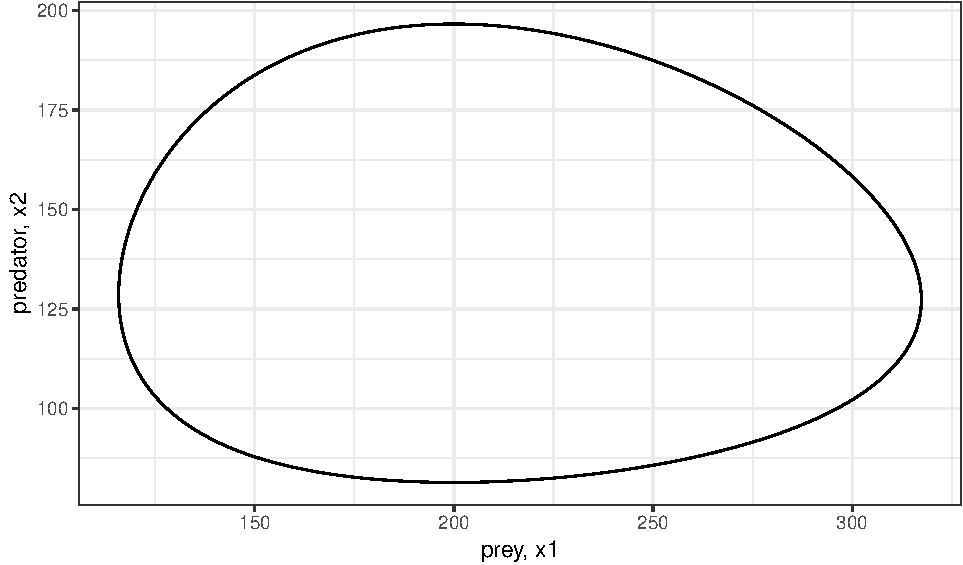
\includegraphics{myDissertation_files/figure-latex/pp1Period-1.pdf}
\caption{\label{fig:pp1Period}Phase space plot of two-species Lotka-Volterra
predator-prey system over a single period (\textasciitilde{}11.145 time
units.}
\end{figure}
\subsection{Concepts behind the
calculations}\label{concepts-behind-the-calculations}

Although the numerical steps for calculating the derivatives-based FI
are relatively straightforward, the concepts required to interpret the
measure in the context of multiple variables is more complex. Here, we
thoroughly discuss the concepts and assumptions behind FI calculation.
Below, steps do not represent steps within the calculation, they
represent the major concepts required

\subsubsection{\texorpdfstring{\textbf{Step 1. Probability of observing
the system in a particular state,
\(p(x)\)}}{Step 1. Probability of observing the system in a particular state, p(x)}}\label{step-1.-probability-of-observing-the-system-in-a-particular-state-px}

Fisher Information (FI) is defined with respect to a probability
distribution. In the derivatives-based method, FI is calculated for a
probability of observing a system (as defined by one or more state
variables) in a particular state, \(p(x)\), over some period of time,
(\(0 to t_{end}\)). In other words \(p(x)\) is the probability that, at
a specific point in time (\(t_{obs}^*\)) we will observe the system in a
particular state, \(x^*\). The time at which we observe the system is a
random variable, \(t_{obs} ~ Uniform(0,t_{end})\). To be clear, the
study system is assumed to be deterministic and we assume no observation
error, however, the observed state of the system, \(x(T_{obs})\), is a
random variable because it is a function of the random observation time,
\(x^*= x(t_{obs}^*)\). The state of the model system, x, is defined in
two dimensions by the number of predators and the number of prey
\eqref{eq:predprey} and is easily visualized
\ref{fig:pp1Period}.Therefore, the probability of observing a particular
state is a two-dimensional joint distribution \ref{fig:2d-hist}.
\begin{figure}
\centering
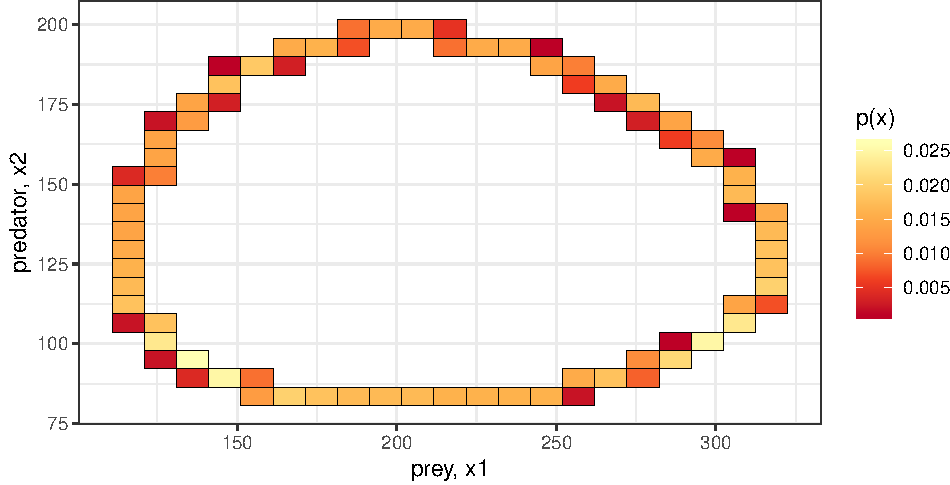
\includegraphics{myDissertation_files/figure-latex/2D-hist-1.pdf}
\caption{\label{fig:2D-hist}A 2-dimensional histogram of the probability of
observing a system in a particular state, \(p(x)\), of the 2-species
Lotka-Volterra predator prey system over a single period
(\textasciitilde{}11.145 time units).}
\end{figure}
A single state of the model system is defined by the number of predators
and prey at a given point in time such that for any given point in time
\(x(t)=[x_1 (t),x_2 (t)]\). At some random time between 0 and
\(t_{end}\) {[}\(T_{obs} ~ Uniform(0,t_{end})\){]} we can count the
number of predators and the number of prey to determine the state of the
model system. We must assume the system is deterministic and there is no
observation error. We can then calculate the probability of observing a
particular predator and prey abundance combination, \(p(x)\). Under
these assumptions, the only possible states of the system are defined by
the system's observed trajectory, the model parameters, and the initial
conditions. Therefore, the support of the probability distribution
\ref{fig:2D-hist} is the trajectory of the system.
\begin{figure}
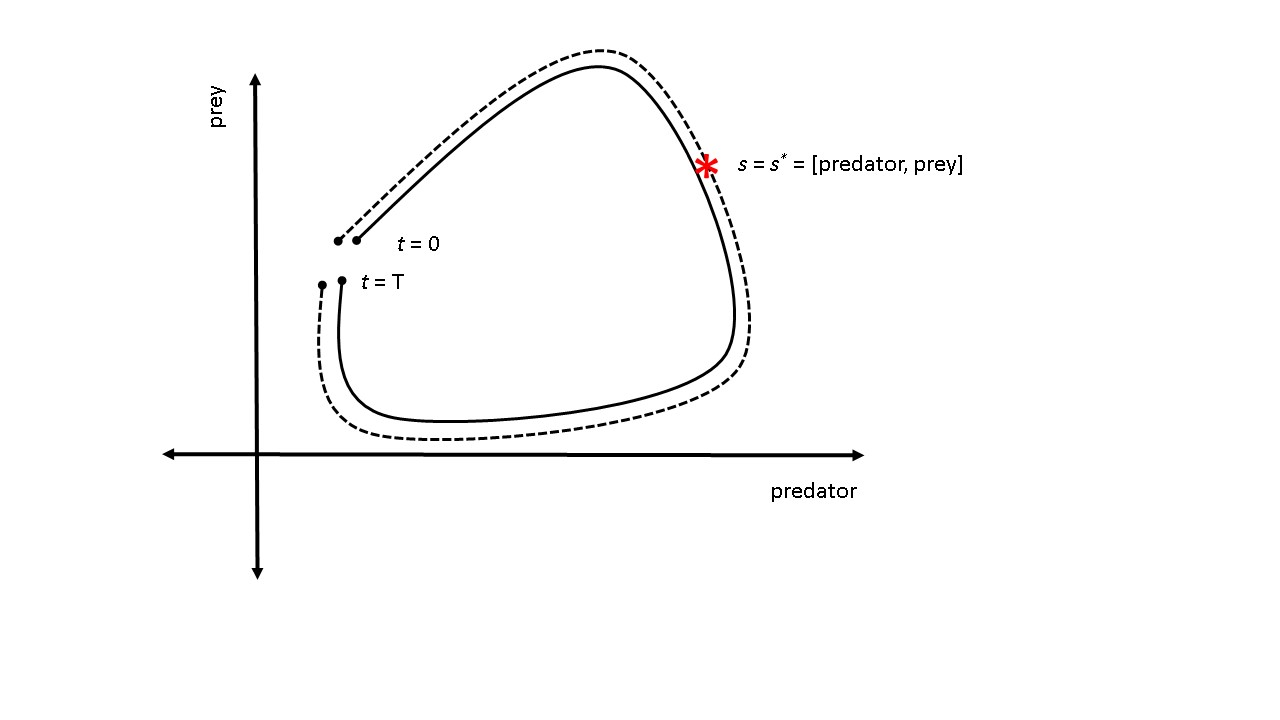
\includegraphics[width=1\linewidth]{./chapterFiles/fiGuide/figures/stringFig} \caption{A single cycle of a hypothetical two-species system over time period $t = 0$ to $t = T$. $s^*$ is the state of the system at some point in time. The dotted line represents the distance travelled by the system in phase space over its trajectory during time $(0, T)$.}\label{fig:stringFig}
\end{figure}
\subsubsection{\texorpdfstring{\textbf{Step 2.} Distance traveled by the
system,
\(s\)}{Step 2. Distance traveled by the system, s}}\label{step-2.-distance-traveled-by-the-system-s}

Distance traveled by the system, s. We can now move from an
n-dimensional representation of the probability distribution to a
one-dimensional representation. To better understand this, imagine
placing a string over the path of the entire trajectory from
\(0 to t_{end}\) \ref{fig:stringFig}. If we know the number of predators
and prey at a particular point in time \((t_{obs}^*)\) then we can mark
that location on the string (see asterisk in \ref{fig:stringFig}. Next,
imagine picking up the string and laying the string flat along a ruler.
The length, s, of the entire string measures the total distance traveled
by the system in phase space. The mark we made on the string (denoted
\(*\)) lies at a distance \(s^*\) between 0 and \(s\). We call this
length the distance traveled by the system, \(s^*\). In this context,
\(s^*\) in phase space represents a measure of cumulative change in
state. We note that the distance traveled in phase space increases
monotonically with time. If the system never revisits the same state
(i.e., the trajectory never overlaps or intersects itself), then every
unique system state (i.e., point on the trajectory) is mapped to a
unique value of distance traveled. Therefore, \(p(x)\) (n-dimensional)
is equivalent to the probability that the system is at distance s, i.e.,
\(p(x)=p(s)\), (where \(p(s)\) is one dimensional; Cabezas, Pawlowski,
Mayer, \& Hoagland (2005)). However, if the system revisits previous
states, then a unique system state may be mapped to different values of
distance traveled and the relationship between \(p(x)\) and \(p(s)\) is
not one-to-one. We calculated the distance traveled s of the model
system over a single cycle (11.145 time units; \ref{fig:distSpeedAccel}.
\begin{figure}
\centering
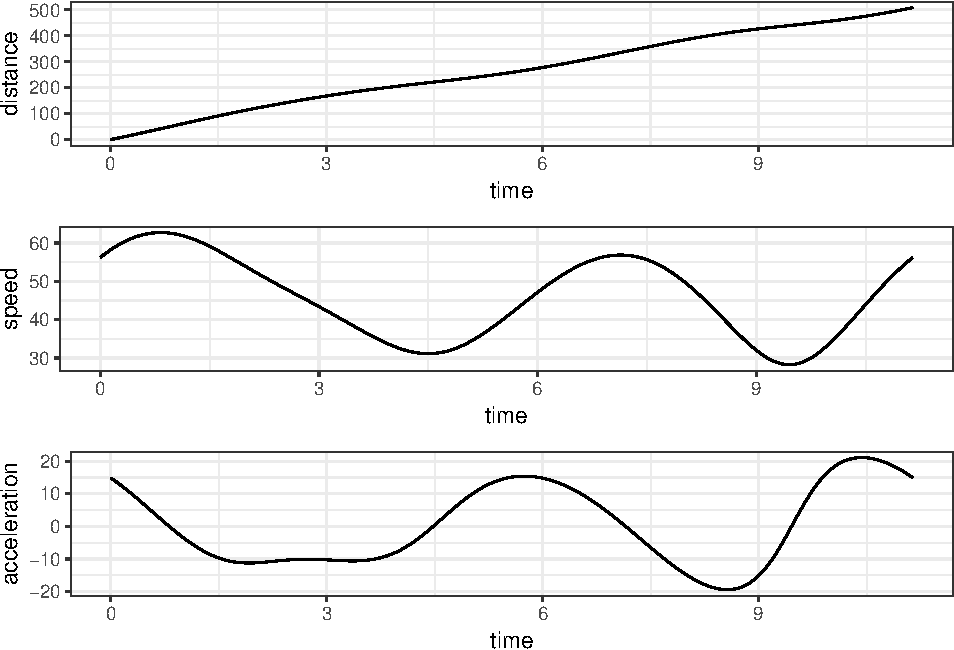
\includegraphics{myDissertation_files/figure-latex/distSpeedAccel-1.pdf}
\caption{\label{fig:distSpeedAccel}From top to bottom, distance traveled in
phase space, speed tangential to system trajectory, acceleration
tangential to system trajectory.}
\end{figure}
\subsubsection{\texorpdfstring{\textbf{Step 3.} \(p(s)\) as a function
of the rate of change of
\(s\)}{Step 3. p(s) as a function of the rate of change of s}}\label{step-3.-ps-as-a-function-of-the-rate-of-change-of-s}

In previous presentations of FI, the relationship between the state of
the system (n-dimensional) and the distance traveled (1-dimensional) was
not always emphasized (Cabezas \& Fath, 2002). Here we use x to denote
the state of the system and s to denote the distance traveled to
emphasize this distinction. If a system travels at a constant speed over
the entire time period, then the system is equally likely to be in any
state along the trajectory (\(s\) is linear and \(p(s)\) is uniform).
Referring to our model system, if the number of predators and prey are
linearly related, then the speed of the system is constant. For
non-linear systems, the distribution above the string will not be
uniform \ref{fig:stringFig}. Rather, it will change depending on the
amount of time the system spends in each state. It follows that \(p(s)\)
is proportional to the inverse of the rate of change of distance
traveled (i.e., the speed along the path in phase space).

We will now demonstrate this using our model system as an example.
Suppose the abundances of the predator and their prey in our model
system predictably operate at carrying capacity. Over a relatively short
period of time the prey abundance quickly declines after a severe
weather event (a pulse disturbance; (Bender et al. 1984), but quickly
recovers. Intuitively, the absolute rate of change at time points near
the disturbance will be larger than during time periods long before or
long after the disturbance. It is therefore more likely that the system
will be (observed) in a state where prey and predators are operating
approximately at carrying capacity than in a state with relatively low
prey abundance. Mathematically, the time, \(t*\), at which we calculate
the abundances of prey and predators is a uniform random variable, and
the distance traveled by the system, \(s^*\), is a function of time, is
differentiable, and monotonically increases. Therefore, the probability
density function of the distance traveled
\(p(s)=\frac{1}{T}\frac{1}{s'}\), where \(s'= \frac{ds}{dt}\) is the
speed of the system (the speed tangential to the trajectory; the first
derivative of the distance traveled; instantaneous rate of change of
\(s\)). We calculated the speed (the first derivative;
\ref{fig:distSpeedAccel} and acceleration (the second derivative;
\ref{fig:distSpeedAccel} of the distance traveled s by the model system
over a single cycle using function ode in package deSolve (Soetaert et
al. 2010) in Program R (R Core Team 2016).

\subsubsection{\texorpdfstring{\textbf{Step 4.} Calculate the
derivatives-based Fisher
Information}{Step 4. Calculate the derivatives-based Fisher Information}}\label{step-4.-calculate-the-derivatives-based-fisher-information}

Now that we understand how to calculate both the distance traveled,
\(s\), and its probability density, \(p(s)\), calculating the
derivatives-based FI is straightforward and computationally inexpensive
\eqref{eq:fiDerivs}. There are several comparable equations for
calculating the shift-invariant FI, and some may offer numerical
advantages over others. Equation \eqref{eq:fiAdapted} is the general form
and Equation \eqref{eq:fi73c} is the amplitude form for FI (in D. A. L.
Mayer et al. (2007), respectively). Although these formulations are
equivalent, \eqref{eq:fi73c} is most readily calculated when the
differential equations for the system are known, obviating any advantage
of a model-free metric.
\begin{equation}   
    I = \frac{1}{T} \int_0^T dt\left[\frac{s''^2}{s'^4}\right]^2 \\  
  \label{eq:fiDerivs}  
\end{equation}
\begin{equation} 
    I = \int \frac{ds}{p(s)}\left[\frac{dp(s)}{ds}\right]^2  \\
    \label{eq:fiAdapted}
\end{equation}
\begin{equation} 
    I = 4 \int ds\left[\frac{dq(s)}{ds}\right]^2 \\
\label{eq:fi73c}
\end{equation}
This article is interested in the Fisher Information calculated for a
distribution of distance traveled, \(s\), by the entire system. We
calculated the Fisher Information value using Equation \eqref{eq:fiDerivs}
over a single period of the model system (\ref{predprey}). We calculated
Fisher Information to be \(5.3\) x \(10^{-5}\) which is consistent with
the results of Mayer et al. (2007).

\section{Case Study}\label{case-study}

Mayer et al. (2007) calculated FI for a predator-prey system for several
discrete values of carrying capacity of prey. The results of this study
showed that FI was different for systems with different carrying
capacities. However, this study did not address the central question of
how FI changes during a regime shift. As an extension of the original
study, we simulate a regime shift by modeling a situation where carrying
capacity is abruptly decreased. To simulate an abrupt change in carrying
capacity, we assume carrying capacity is described by Eq. 6 where \(k1\)
is the initial carrying capacity, \(k2\) is the final carrying capacity,
\(t*\) is the time of the regime shift, and alpha is a parameter that
controls how quickly the regime shift occurs. The hyperbolic tangent
function simulates a smooth, continuous change in carrying capacity
while still allowing for the change to occur suddenly. To incorporate
the change in carrying capacity into the system differential equations
we define the rate of change of carrying capacity as given by
\eqref{eq:mayerCase}.\\
\begin{equation}  
  k(t) = k_1  - 0.5(k_1-k_2)(\tanh(\alpha (t-t^*))+1)     \\
  k'(t) = 0.5\alpha (k_1-k_2)(\tanh(\alpha(t-t^*))^2 +1)      \\ 
\label{eq:mayerCase}
\end{equation}
\begin{verbatim}
[1] 5.370485e-05
\end{verbatim}
\begin{verbatim}
[1] 5.371751e-05
\end{verbatim}
\begin{verbatim}
[1] 5.326461e-05
\end{verbatim}
\begin{figure}
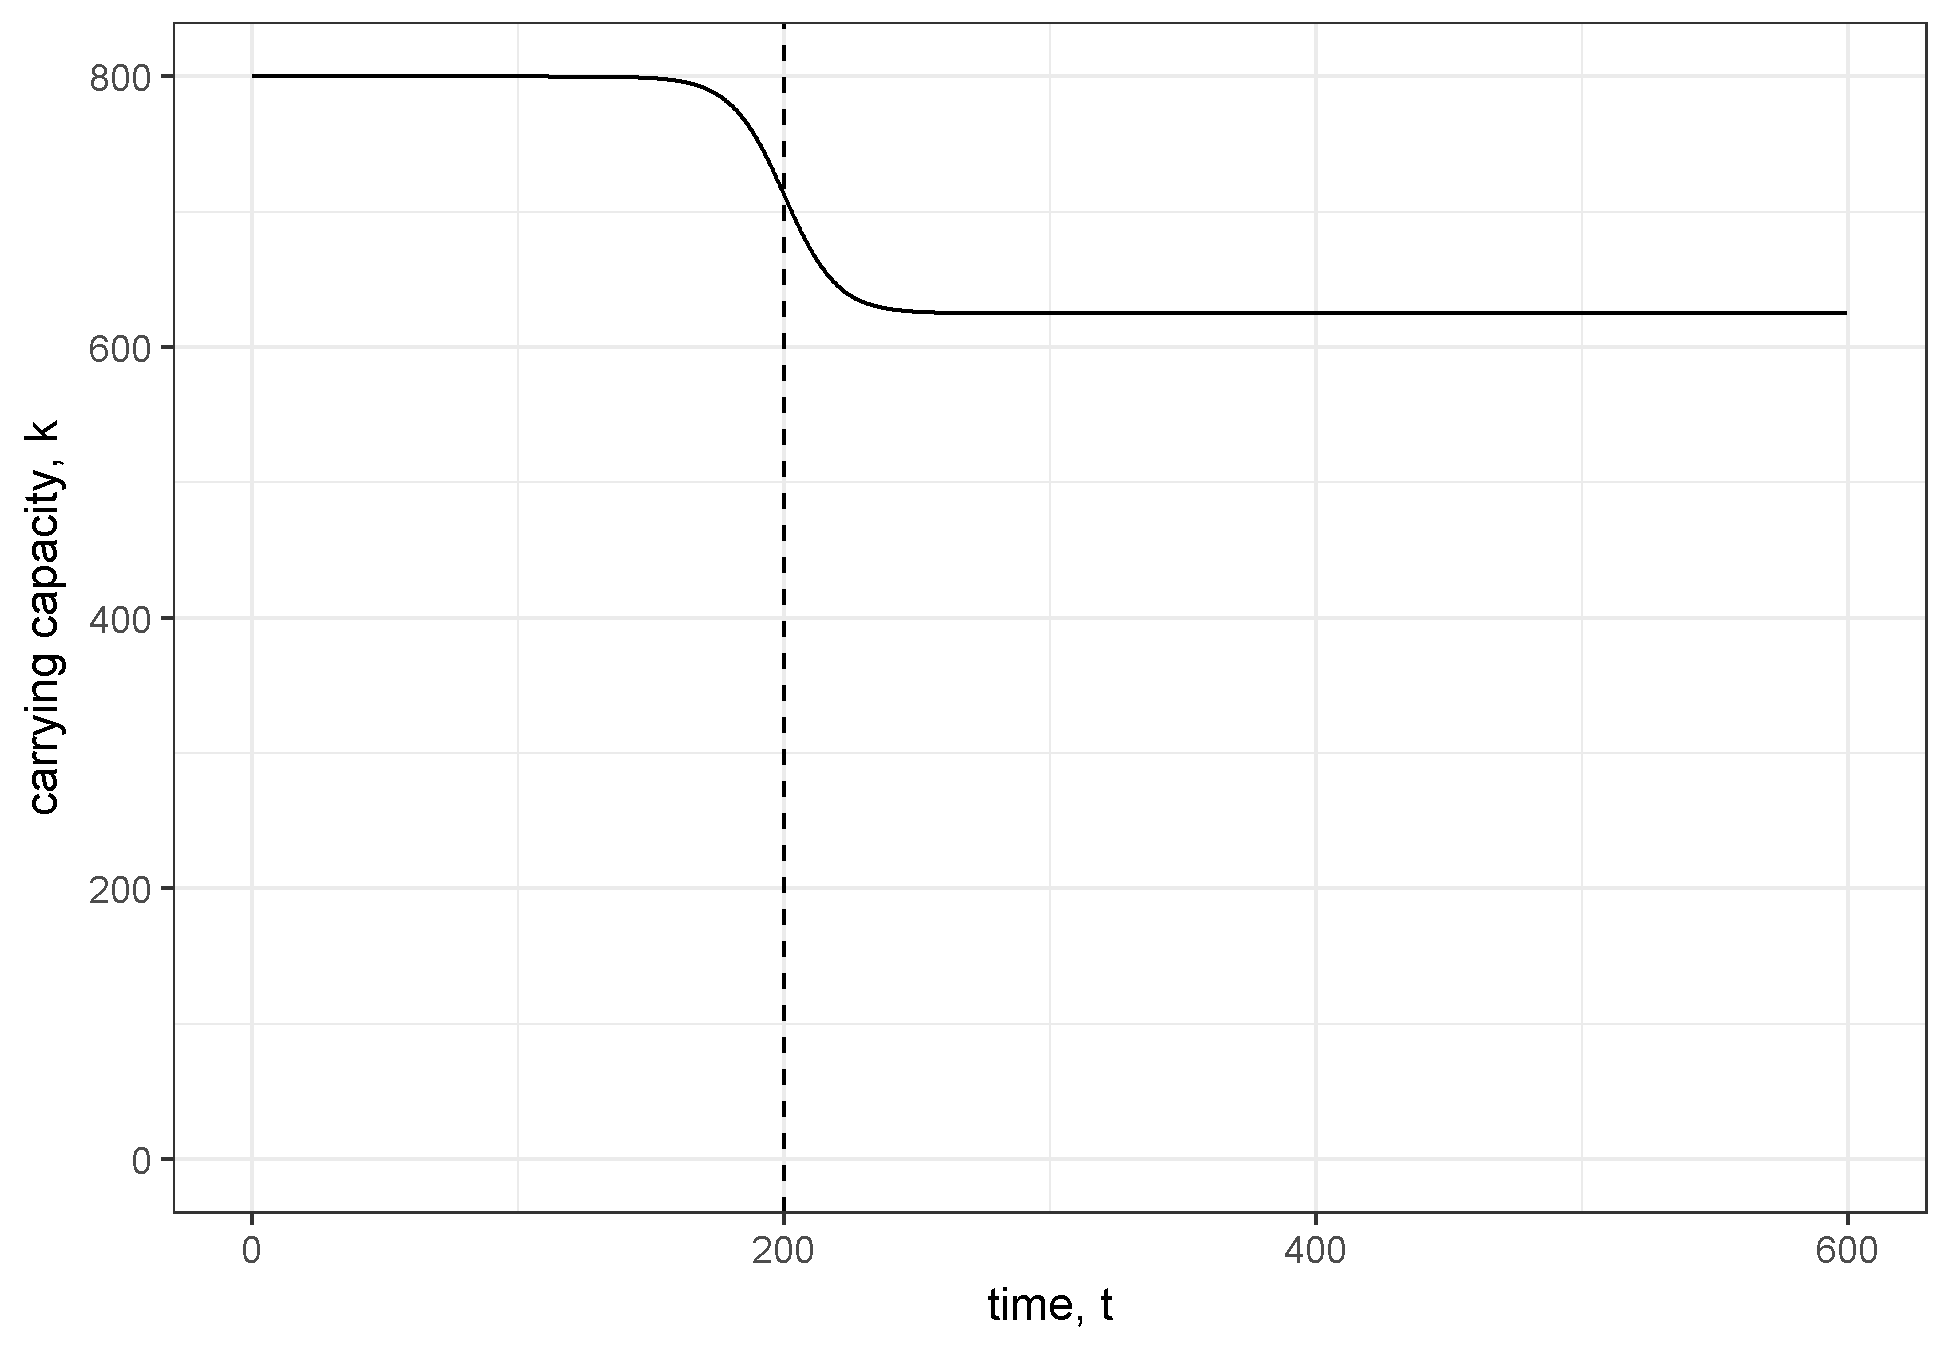
\includegraphics[width=1\linewidth]{./chapterFiles/fiGuide/figures/kByTime} \caption{Carrying capacity over time with a regime shift occuring around time 200.}\label{fig:kByTime}
\end{figure}
\begin{figure}
\centering
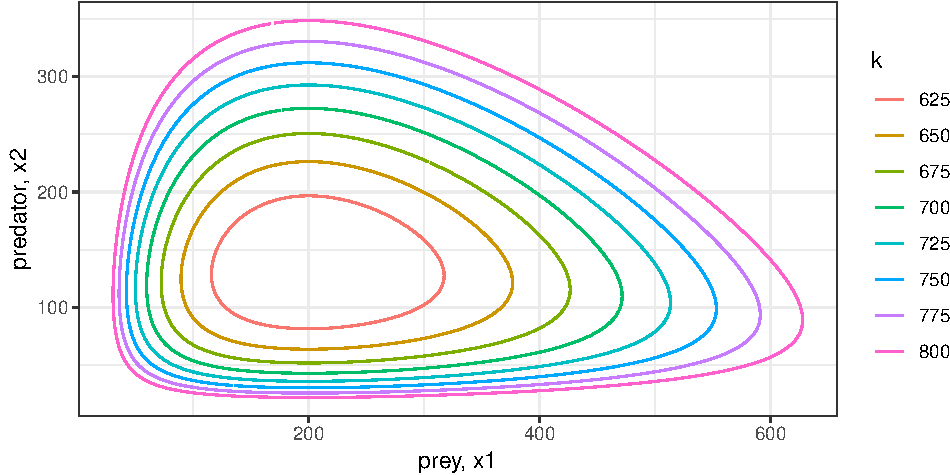
\includegraphics{myDissertation_files/figure-latex/kTrajectories-1.pdf}
\caption{\label{fig:kTrajectories}Phase space plot of system trajectories
for different values of k}
\end{figure}
We assumed an initial carrying capacity of 800 and a final carrying
capacity of 625 which corresponds to the range of carrying capacities
explored by Mayer et al. (2007). We simulated a time series of 600 time
units with a regime change after 200 time units. We used an alpha value
of 0.05. The time series for carrying capacity is shown in
\ref{fig:kByTime} and the system trajectory in phase space is shown in
\ref{fig:kTrajectories}. The distance travelled in phase space (i.e.,
cumulative change in state) is shown in \ref{fig:distOverTime} and the
speed of the system (i.e., rate of change) is shown in
\ref{fig:dsdtOverTime}.
\begin{figure}
\centering
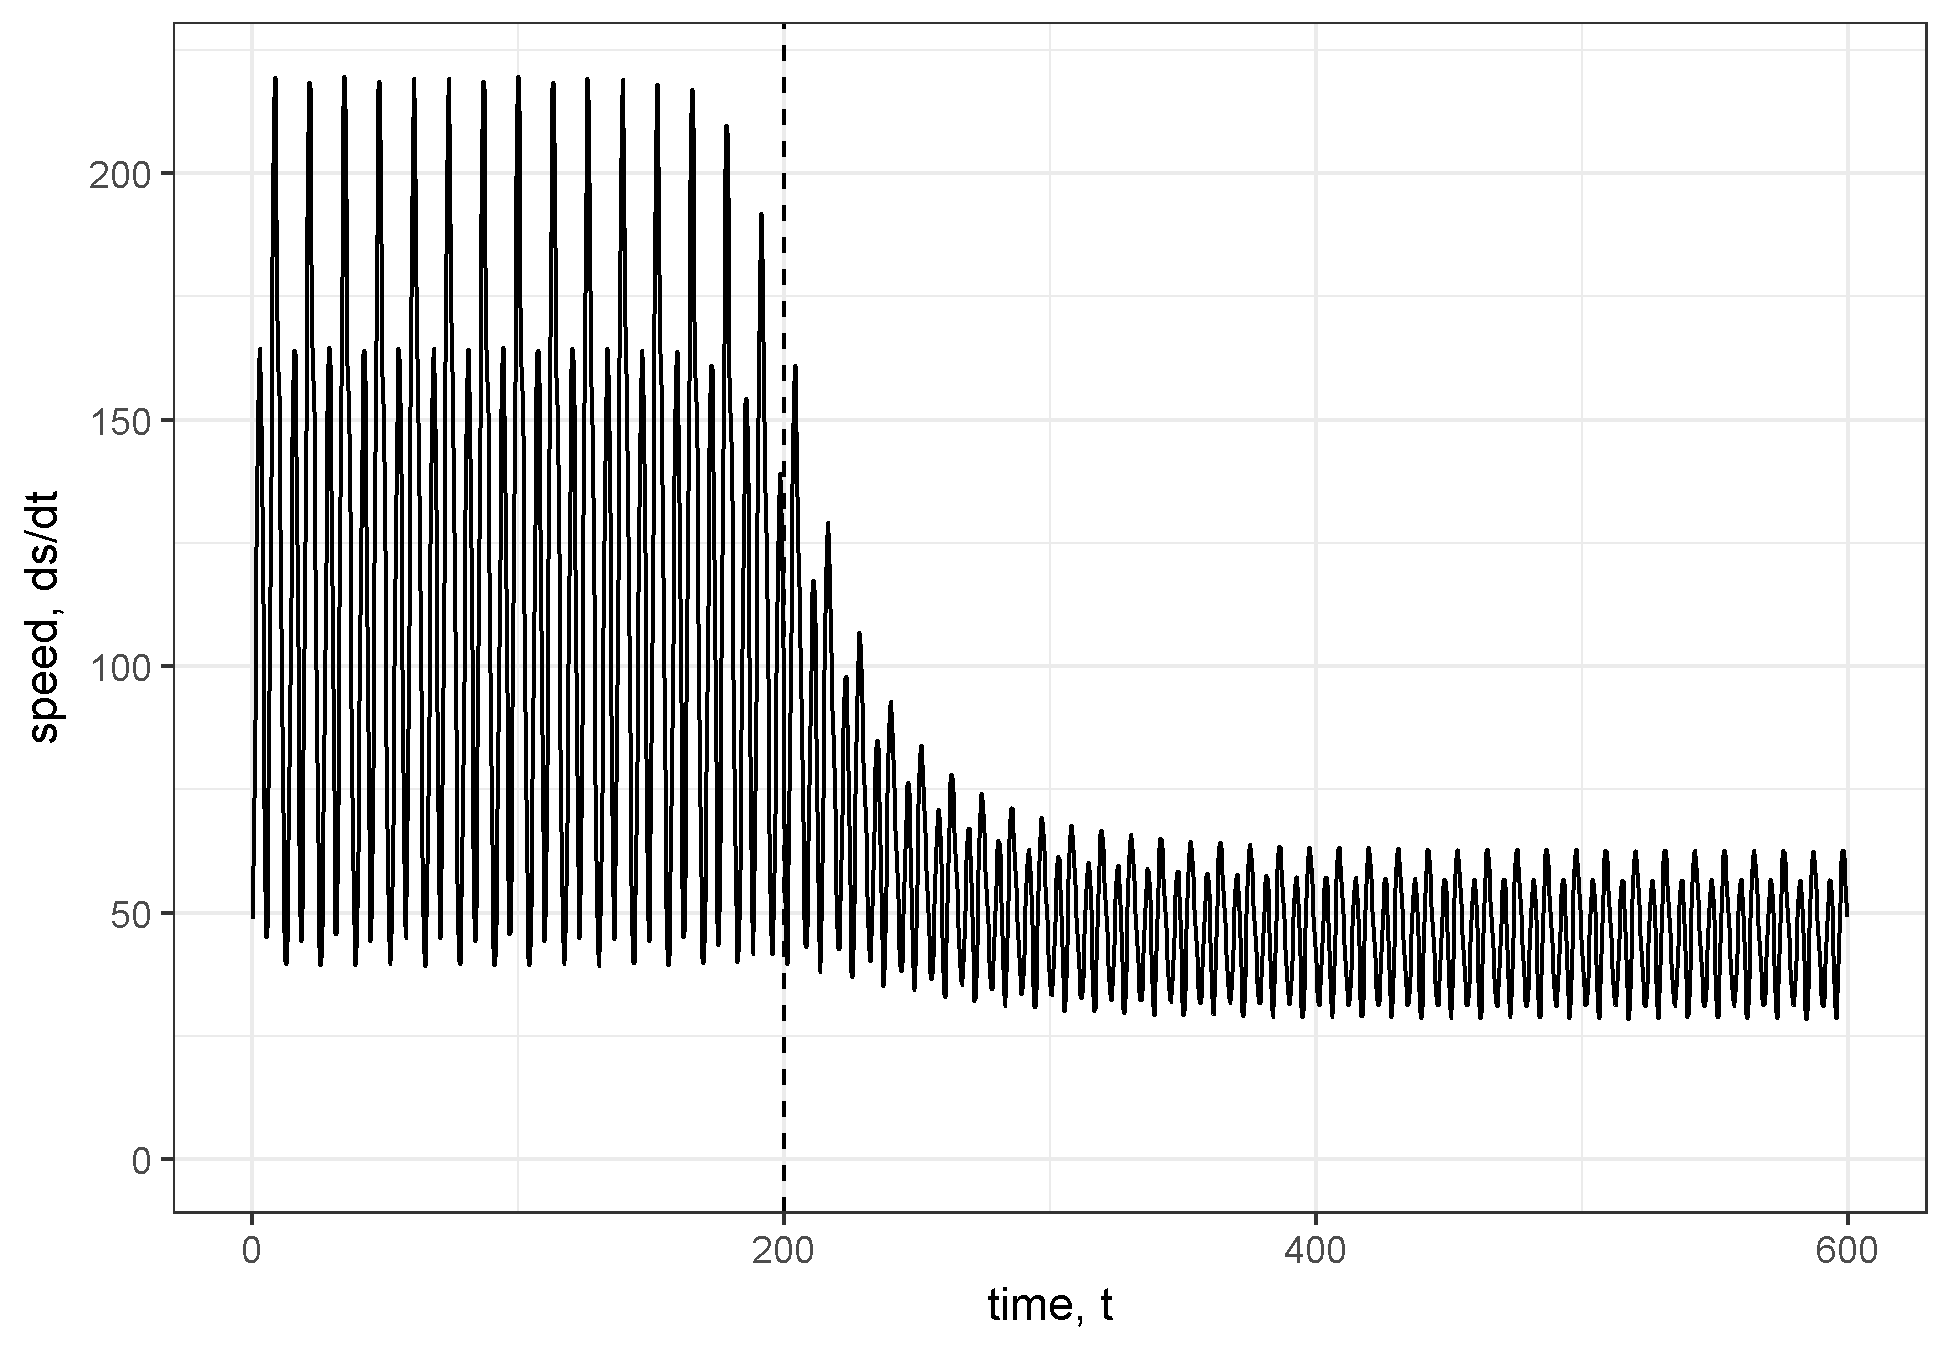
\includegraphics{./chapterFiles/fiGuide/figures/dsdtOverTime.png}
\caption{\label{fig:dsdtOverTime}Speed of the system (rate of change) in
phase space. Dashed vertical line at time 200 indicates location of
regime shift.}
\end{figure}
We calculated FI for the distribution of distance travelled over a
series of non-overlapping time windows. Multiple sources suggest the
length of the time window should be equal to one system period such that
FI is constant for a periodic system (Cabezas \& Fath, 2002; D. A. L.
Mayer et al., 2007). However, the system period is different before,
during, and after the regime shift. Therefore, we performed two separate
calculations of FI using window sizes corresponding to the initial and
final period of the system (\(13.061\) and \(11.135\), respectively).
The change in FI over time is shown in \ref{fig:fiOVerTime}.
\begin{figure}
\centering
\includegraphics{./chapterFiles/fiGuide/figures/fiOverTime.png}
\caption{\label{fig:fiOverTime}Fisher Information calculated for
non-overlapping time windows. Two different window sizes were used as
indicated by color. Dashed vertical line at time 200 indicates
approximate location of regime shift.}
\end{figure}
\section{Conclusions}\label{conclusions}

We simulated a regime shift caused by a change in carrying capacity
(\(K\)) within a simulated, two-species Lotka-Volterra system. We
applied the Fisher Information (FI) method for regime shift detection to
the simulated time series data. The predator-prey system was modeled as
deterministic and the time series data was free from measurement and
observation error. Despite this, the estimated FI had high variation
over time, and results were dependent on the size of the time window
used (winsize) in the calculation \ref{fig:fiOVerTime}. The FI method
for regime shift detection is based on the cumulative change in the
state of the system (i.e., distance traveled in phase space) and the
rate of change of the system (i.e., speed tangential to trajectory in
phase space). The distance travelled metric, \(s\), and its speed,
\(dsdt\), appear better visual indicators of the regime shift than FI
{[}\ref{distOverTime}; \ref{dsdtOverTime}{]}.

In our explanation of the FI concept and calculation, we emphasize the
distinction between the \emph{state of the system} and the
\emph{distance traveled in phase space}. There are several reasons worth
emphasizing this. First, there may not always be a one-to-one
relationship between the probability of observing a system in a
particular state and the probability of observing a system at a
particular distance along the trajectory. In these situations the
interpretation of FI may be less clear than if a one-to-one relationship
existed. Second, this distinction facilitates the separation of the
dimensionality reduction step (calculating distance traveled in phase
space, \(s\)) from the subsequent steps related specifically to FI.
Third, the distinction suggests that the \textbf{value of FI as a regime
shift detection method is related to the rate of change of the system}
(i.e., velocity and acceleration tangential to system trajectory in
phase space). In particular, the distribution for which FI is calculated
is simply the distribution of the distance traveled in phase space, when
time is assumed to be uniformly distributed over a given interval.

Our results suggest that insights can be gained directly from the
calculation of distance traveled and associated rates of change.
Consequently, these insights preclude the need to calculate beyond Step
3 (described above). This result also supports the use of the distance
travelled metric, or the derivatives-based Fisher Information
\label{eq:fiDerivs}.

One remaining issue that is prevalent across ecological field studies is
the assumption that the system is observed without error. Although
ecological data rarely fulfill this assumption, this does not suggest
that FI is useless as a metric of system stability. The primary
difficulty with noisy data, especially with observations in integer form
(e.g.~count data), is that the denominator in can easily be zero for
some pair of observations, making FI an infiniate value within windows
which contain two or more adjacent zero observations. One possible
solution is to smooth the multidimensional vector of observations prior
to calculating the derivatives, or to treat any sequential identical
value as missing, and simply use a larger time step for that portion of
the window calculation.

The utility of Fisher Information in ecological studies is also stunted
by its interpretability. This metric is unitless, making its values
relative only within-sample (e.g., within a single time series).
Further, interpreting the results within-sample is currently a
qualitative effort (Mantua, 2004, Fath et al. 2003). When the FI of a
system is increasing, the system is said to be moving toward a more
orderly state, and most presentations of FI posit sharp changes in FI,
regardless of the directionality of the change, may indicate a regime
shift (Cabezas \& Fath, 2002; Karunanithi et al., 2008; Spanbauer et
al., 2014). Due to the qualitative nature of these interpretations of
Fisher Information, intimate knowledge of the system in question and the
potential driver(s) of the observed regime shift are required to confirm
presence of a shift.

\section{Acknowledgements}\label{acknowledgements-1}

We thank H. Cabezas and B. Roy Frieden for early discussions regarding
the development of Fisher Information. This work was funded by the U.S.
Department of Defense's Strategic Environmental Research and Development
Program (project ID: RC-2510).

\chapter{An application of the Fisher Information binning method to
spatiotemporal avian community
data}\label{an-application-of-the-fisher-information-binning-method-to-spatiotemporal-avian-community-data}

\section{Abstract}\label{abstract-1}

\section{Introduction}\label{introduction-2}

Numerous quantitative methods are proposed for identifying abrupt
changes in ecological systems. Despite advances in the detecting regime
changes in atmospheric, oceanic, and aquatic systems, it still poses
difficult to identify abrupt changes in complex terrestrial ecological
systems (Scheffer et al. 2009). Few studies have rigorously tested the
quantitative regime shift detection methods using observational data
from real, ecological systems (Bestelmeyer et al. 2011). Many of the
advances in ecological regime shift detection theory have been made in
the aquatic sciences (freshwater and marine, but especially freshwater
lakes; see Carpenter et al. 2011, Batt et al. 2013). However, many of
the methods (e.g., critical slowing down, variance, autoregression)
which appear to be useful in aquatic systems do not readily translate to
larger, more complex, terrestrial systems. Additional quantitative
methods have been proposed in the ecological literature for handling
observations from more complex systems (see @ref:(review)). Applications
of these quantitative methods to real systems data, coupled with expert
knowledge, are required to advance regime change theory.

Leading indicators of regime shifts using univariate data are
well-tested on both theoretical and empirical data (e.g.~Burthe et al.,
2015). Commonly used indicators applied to time-series data include an
index of variance, moments around the grand mean (skewness and
kurtosis), and critical slowing down (Brock and Carpenter 2006).
Although univariate indicators may provide insight into relatively
simple systems, like small lakes and isolated wetlands (carpenter
references), their reliability as indicators for complex systems is less
certain. Leading indicators can be a reliable warning of impending shift
(@carpenterBrock2006), however, may prove most useful in systems of
which we have mapped the suspected drivers and response mechanisms
(Scheffer et al. 2009). Some methods have beeen adapted for spatially
explicit data (Butitta et al 2017; Kefi et al. 2014). Some methods have
been applied to early-warning indicators in whole systems (Carpenter et
al. 2011), however, it is uncommon to have enough information to build
reliable networks or food webs. Consequently, reliably measuring the
ecological system at hand is often realistically (and financially) not
possible.

Contrary to univariate indicators of regime change, the Fisher
Information measure is proposed as a method for identifying changes in a
multivariate data set (Fisher 1922, Cabezas and Fath 2002, Karunanithi
et al. 2008, Eason and Cabezas 2012, Eason et al. 2014, Ahmad et al.
2016). See Chapter \{\#derivatives\} for a detailed explanation of the
concept of Fisher Information. It is suggested that Fisher Information
captures the ecological complexity of a system if given a set of
observations which encompass the ecological drivers which dictate the
state of the system. A relatively rapid change in the amount of Fisher
Information is interpreted as a change in system configuration or
orderliness (e.g., see Karunanithi et al. 2008). Fisher Information is
rooted in statistics and in the physical sciences-it has only recently
been applied to complex ecological and social-ecological systems
(Frieden 1998; Fath et al.; Palowski et al). Despite its established use
in identifying the degree of predictability of closed systems in
physics, Fisher Information's utility in rigorously and universally
assessing the state of complex ecological systems is not known.

In this chapter I present an application of the Fisher Information
measure using what I call the `binning' Fisher Information method (first
proposed in \{Karunanithi et al. (2008)\}; hereafter, binning method) to
a broad-scale and long-running abundance time series in North America. I
present both spatial and temporal applications of the Fisher Information
measure to community data to provide an applied and baseline
understanding of how the Fisher Information binning measure appears on
these data. This chapter also serves as an exploratory study of the
Fisher Information binning measure for identifying regime boundaries and
change in both space and time.

\section{Methods}\label{methods-1}

\subsection{Data collection}\label{data-collection}

I use community abundance data from long-term monitoring programs to
identify spatial and temporal regimes using the Fisher Information
binning method. Although Fisher Information can be calculated using any
number of variables, the binning method (see \ref{derivatives}) requires
many data points and a large number of observations at each sampling
site or period of time. I therefore chose to using breeding bird
abundances from a long-standing avian community survey, the North
American Breeding Bird Survey (NABBS) (({\textbf{???}})). The NABBS
annually collects data during the breeding season using a standardized
roadside, single observer point count protocol and has been collecting
data regularly across North America since 1966. Despite its protocol of
annual collection at 50 stops on an approximately 24.5 mile stretch of
rural roads) the reliance on volunteers to collect the data results in
some routes not being covered in some years. Routes are necessarily
added or discontinued, and some routes are not sampled in a given year.
As such, sites may have missing observations and are treated as such.

Although data missingness does not prevent calculation of the Fisher
Information binning measure the effect(s) of missing data on the
calculation and interpretation of this measure are largely unknown. For
this reason I analyze only sampling sites (for temporal analyses) or
spatial transects (for spatial analyses) which have at least 15 years
(temporal) or 15 sites (spatial) to avoid potential effects of missing
data on the calculation of the Fisher Information.

\subsection{Study areas}\label{study-areas}

Although the NABBS conducts surveys throughout much of North America, I
limit my analyses to the continental United States and parts of southern
Canada. NABBS coverage of the boreal forests of Canada are sparse in
space, and many routes in Mexico have fewer than 25 years of
observations. I identified two strip-transects across large swaths of
the continental United States-one running in a South-North direction,
the other running East-West-and two individual NABBS sites (routes) to
conduct spatial and temporal regime shift analyses, respectively. The
South-North and East-West transects are hereafter referred to as spatial
transects, and the NABBS sampling sites are referred to as routes (see
section `Building spatial transects', below).

\subsubsection{Military bases as study
sites}\label{military-bases-as-study-sites}

The Mission of the US Department of Defense is to provide military
forces to deter war and protect the security of the country, and a
primary objective of individual military bases is to maintain military
readiness. To maintain readiness, military bases strictly monitor and
manage their natural resources. Military bases vary in size and nature,
and are heterogeneously distributed across the continental United States
(See \ref{fig:ewRouteMap}). The spread of these bases, coupled with the
top-down management of base-level natural resources presumably
influences the inherent difficulties associated with collaborative
management within and across military bases and other natural resource
management groups (e.g., state management agencies, non-profit
environmental groups.

Much like other actively managed landscapes, miltiary bases are
typically surrounded by non- or improperly-managed lands. Natural
resource managers of military bases face environmental pressures within
and surrounding their properties, yet their primary objectives are very
different. Natural resource managers of military bases, whose primary
objective is to maintain military readiness, are especially concerned
with if and how broad-scale external forcings might influence their
lands. Prominent concerns include invasive species, wildlife disease,
and federally protected species (personal communication with Department
of Defense natural resource managers at Eglin Air Force and Fort Riley
military bases). For these reasons, natural resource managers attempt to
create buffers along their perimeters (e.g., live fire/ammunitions
suppression, wide fire breaks). Identifying the proximity of military
bases to historic and modern ecological shifts may provide insight into
the effectiveness of their natural resource management efforts.

\subsubsection{Focal military bases}\label{focal-military-bases}

The NABBS routes chosen for analyses in this Chapter lie within or near
two two US Department of Defense properties: Fort Riley military base
(located at approximately 39.110474 ??, -96.809677 ??; Kansas, USA) and
Eglin Air Force base (located at approximately 30.459588 ??, -86.548459
??; Florida USA). These military bases were used for research conducted
under the a grant funded by the Department of Defense's Strategic
Environmental Research and Development Program (SERDP; RSCON-15-01:RC
3150).

Eglin Air Force and Fort Riley military bases serve as ideal reference
sites for this study. The natural resource management teams are active
on each base and have been for at least two decades and each uses
wildfire as a management technique. Fort Riley military base is
especially relevant to regime shift detection method exploratory
analysis. Woody encroachment of the Central Great Plains over the last
century has triggered shifts in dominant vegetative cover and diversity
(Ratajczak et al. 2012) in the area surrounding Fort Riley military base
(e.g., Van Auken 2009). This phenomena should present itself as a regime
boundary should Fisher Information be a robust regime shift detection
method. Eglin Air Force base is embedded within a heavily developed
matrix, and consequently has experienced less pronounced effects at
broad spatial extent and over longer periods. Therefore, the ecological
communities (and the data) surrounding Eglin Air Force base may exhibit
a greater amount of noise, making the effect size of a regime shift and
consequently the effect size smaller and more difficult to detect. For
these reasons, Eglin Air Force and Fort Riley military bases are ideal
locations for an exploratory analysis of the Fisher Information binning
method as a regime shift detection method.
\begin{figure}

{\centering 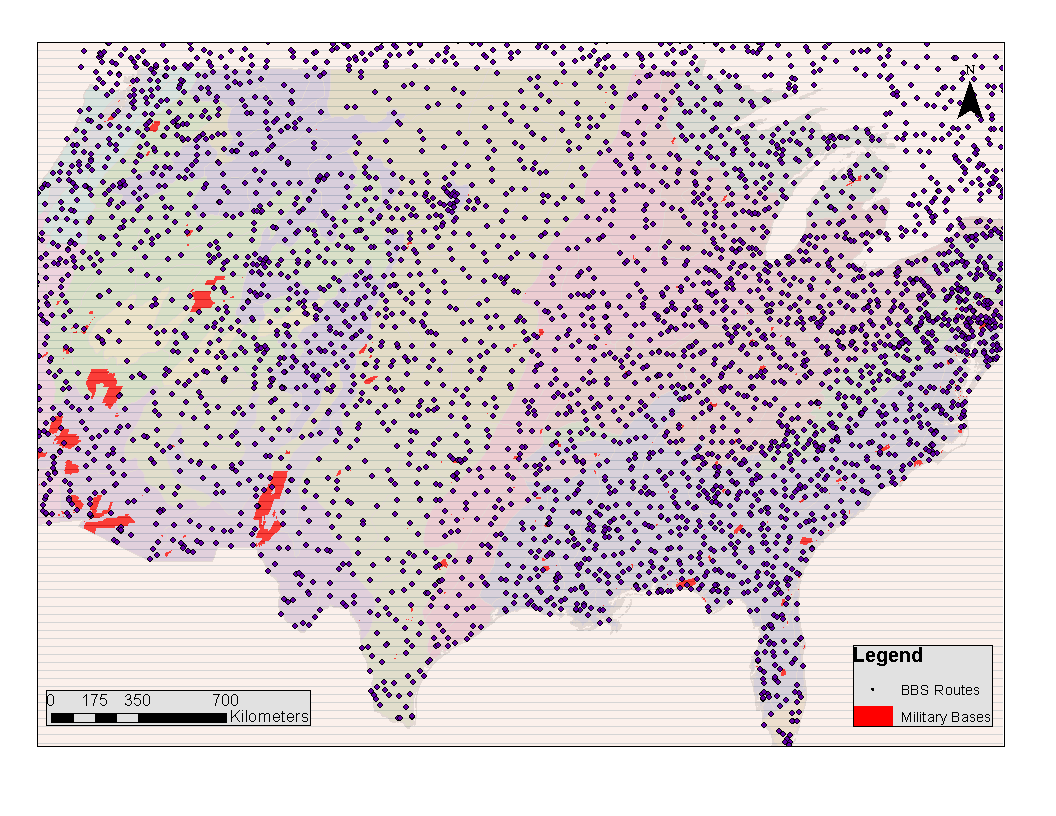
\includegraphics{chapterFiles/binningChap/figures/bbsPoints} 

}

\caption{Transect sampling design of East-West-running transects used to identify spatial regime boundaries.}\label{fig:bbsPoints}
\end{figure}
\subsubsection{Delineating spatial transects for spatial
analysis}\label{delineating-spatial-transects-for-spatial-analysis}

To our knowledge, Sundstrom et al. (2017) is the only study to use the
Fisher Information binning method on spatially-referenced data. The
authors of this study hand-picked NABBS routes to be included in their
spatial `transect' (see \ref{fig:bbsPoints}a in Sundstrom et al. 2017)
such that each `ecoregion' in their analysis would be similarly
represented by avian community data (via the same number of NABBS route
within each ecoregion). I constructed a gridded system across the
continental United States and Canada to ameliorate potential effects of
site selection bias (see \ref{fig:bbsPoints} for a visualization of the
East-West transect grid sections). The grid system comprised
55-mile-wide transects running in either North-South or East-West
directions. I chose one North-South and one East-West transect based on
which transect encompassed the Eglin Air force and Fort Riley military
bases ( \ref{fig:nsRouteMap} and \ref{fig:ewRouteMap}).
\begin{figure}

{\centering 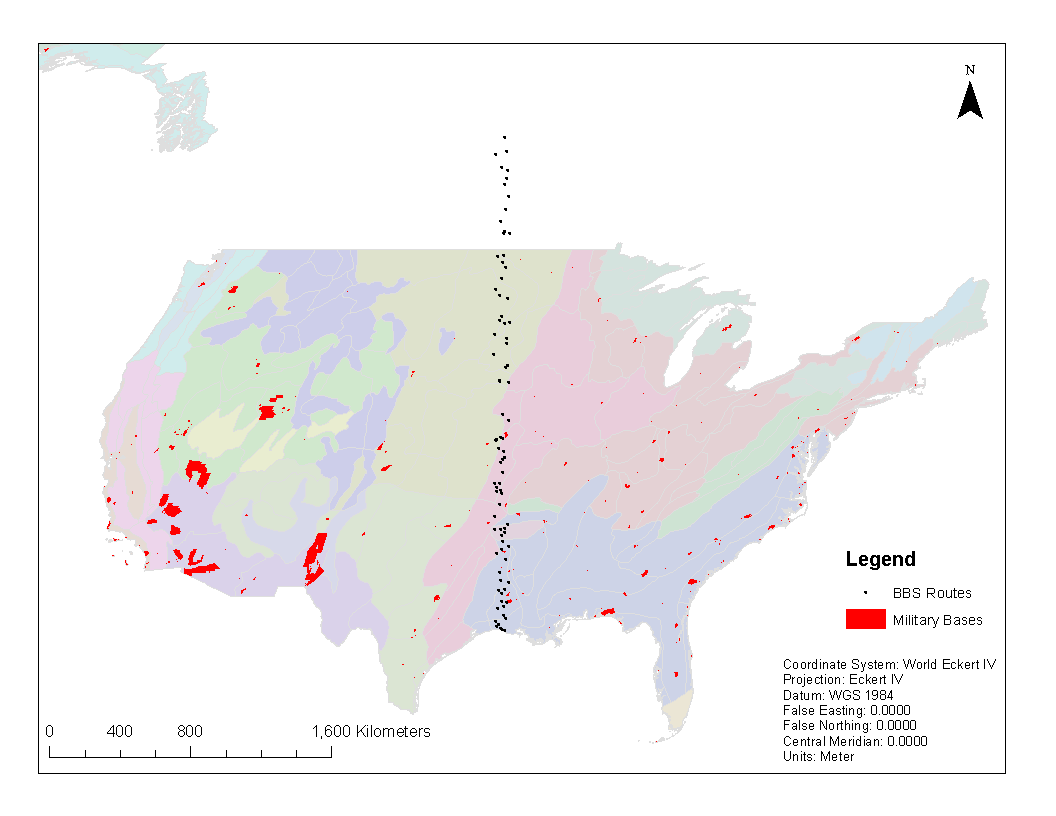
\includegraphics{chapterFiles/binningChap/figures/nsRouteMap} 

}

\caption{A single, North-South transect of Breeding Bird Survey Routes used to calculate the Fisher Information binning measure and univariate early-warning indicators. }\label{fig:nsRouteMap}
\end{figure}\begin{figure}
{\centering 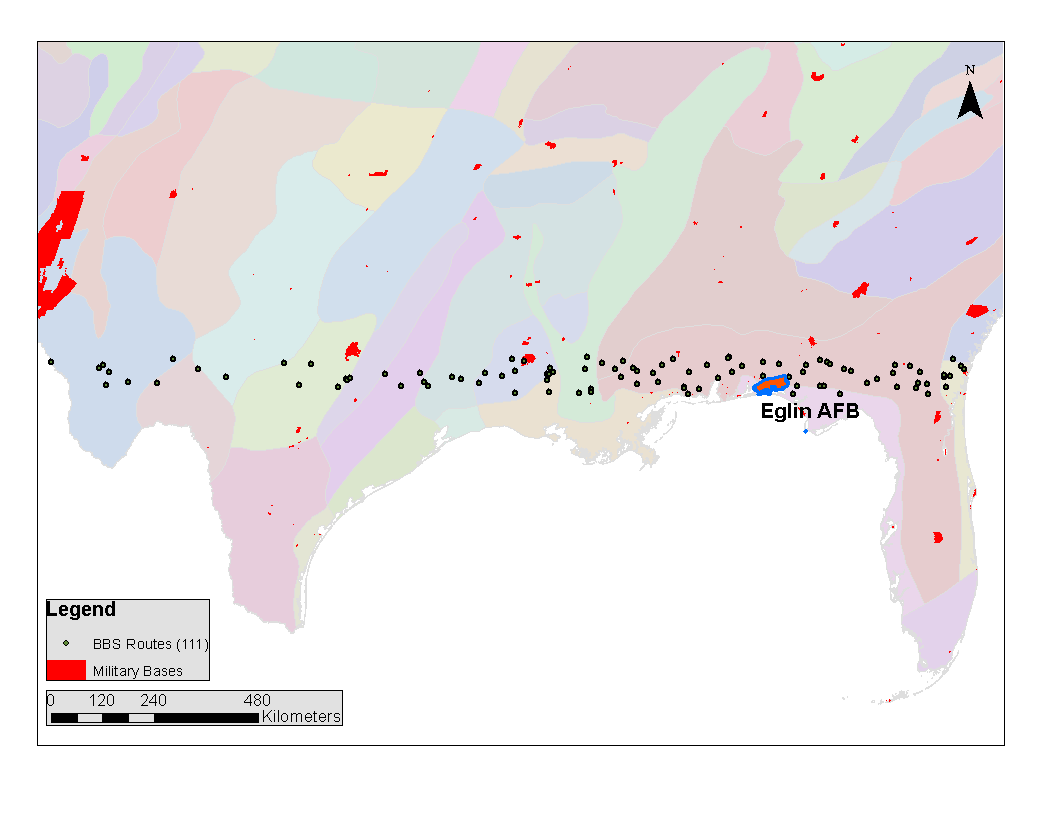
\includegraphics{chapterFiles/binningChap/figures/ewRouteMap} 

}

\caption{A single East-West transect of Breeding Bird Survey routes used to calculate the Fisher Information binning measure. Military base locations can be used to visually estimate the proximity [of Department of Defense properties] to potential regime boundaries.}\label{fig:ewRouteMap}
\end{figure}
\subsubsection{Delineating transects for spatial
analysis}\label{delineating-transects-for-spatial-analysis}

\subsubsection{Selecting routes for temporal
analysis}\label{selecting-routes-for-temporal-analysis}

Temporal analysis consisted of time series of annually collected data at
the level of an individual NABBS route. I analyzed two NABBS routes near
the Eglin Air Force base-one to the East and one to the West.

\subsection{Calculating the Fisher Information binning
measure}\label{calculating-the-fisher-information-binning-measure}

Fisher Information, \(I(??)\), was developed in 1922 by Ronald Fisher as
a measure of the amount of information that an observable variable, X,
reveals about an unknown parameter, \(??\). Fisher Information is a
measure of indeterminacy (Fisher 1922) and is defined as,
\begin{equation} 
I(\theta) = \int \frac{dy}{p(y|\theta)}\left[\frac{dp(y|\theta)}{d\theta}\right]^2
\label{eq:fiGeneral1922}
\end{equation}
where \(p(y|??)\) is the probability density of obtaining the data in
presence of ??. The Fisher Information measure (FIM) is used to
calculate the covariance matrix associated with the likelihood,
\(p(y|??)\). Fisher Information is described as Extreme Physical
Information (EPI; Frieden and Soffer 1995, Kibble 1999, Frieden et al.
2002), a measure that has been used to track the complexity of systems
in many scientific disciplines including, physics, cancer research,
electrical engineering, and, recently, complex systems theory and
ecology

Fisher Information as gathered from observational data provides insight
as to the dynamic order of a system, where an orderly system is one with
constant (i.e., unchanging) observation points, and one whose nature is
highly predictable. A disorderly system is just the opposite, where each
next data point is statistically unpredictable. In ecological systems,
patterns are assumed to be a realization of ecosystem order; therefore,
we should expect orderliness in a system with relatively stable
processes and feedbacks. Orderliness, however, does not necessarily
infer long-term predictability. \eqref{eq:fiGeneral1922} is next adapted
to estimate the dynamic order of an entire system, \(s\), as
\begin{equation} 
I = \int \frac{ds}{p(s)}\left[\frac{dp(s)}{ds}\right]^2
\label{eq:fiAdapted}
\end{equation}
where \(p(s)\) is the probability density for \(s\). Here, a relatively
high Fisher Information value (\(I\)) infers higher dynamic order,
whereas a lower value (approaching zero) infers less orderliness. To
limit the potential values of I in real data, we can calculate the
amount of Fisher Information by re-expressing it in terms of a
probability amplitude function \(q(s)\) (Fath et al. 2003, Mayer et al.
2007, eq. 7.3):
\begin{equation}
I = 4 \int ds\left[\frac{dq(s)}{ds}\right]^2
\label{eq:fiAmplitude}
\end{equation}
A form specific to the pdf of distance travelled is derived as (D. A. L.
Mayer et al., 2007, eq. 7.12)(see @derivatives for more information on
\eqref{eq:derivativesFI}):
\begin{equation} 
\label{eq:derivativesFI}
I = \frac{1}{T} \int_0^T dt\left[\frac{s''^2}{s'^4}\right]^2
\end{equation}
, where T is the number of equally spaced time points over which we
integrate.

These two variants of Fisher Information, \eqref{eq:fiAmplitude} and
\eqref{eq:derivativesFI}, have been used to estimate the dynamic order of
complex systems (Cabezas and Fath 2002, Karunanithi et al. 2008).
Numerical calculation of I using the binning method
(\eqref{eq:fiAmplitude} and \eqref{eq:derivativesFI}) incorporates a binning
procedure for the probability of the system, \(p(s)\), as being in one
of an unidentified number of states (\(s\)).

I carefully considered prior to analyzing data using the Fisher
Infomration binning method \eqref{eq:fiAmplitude}). The binning procedure
allows for a single point in time or space to be categorized into more
than one state, which violating the properties of alternative stable
states theory. The size of states (see Eason and Cabezas 2012) measure
is required to construct p(s). In the case of high dimensional data, a
univariate binning procedure of p(s) is not intuitive (i.e., reducing a
multivariable system to a single probability distribution rather than
constructing a multivariate probability distribution). Importantly, when
using community or abundance data, rare or highly abundant species can
influence the size of states criterion, thus influencing the assignment
of each point into states. Finally, \eqref{eq:fiAmplitude} assumes equal
spacing (in space or time) between sampling points. Each of these
violations can be avoided by using \eqref{eq:derivativesFI}; Cabezas and
Fath 2002, Fath et al. 2003) to calculate the Fisher Information measure
(see @derivatives for discussion on this topic). The derivatives method
(\eqref{eq:derivativesFI}) estimates the trajectory of the system's state
by calculating the integral of the ratio of the system's acceleration
and speed in state space (Fath et al. 2003).

\section{Results}\label{results-1}

\subsection{Temporal data}\label{temporal-data}

\subsection{Spatial data}\label{spatial-data}

\subsection{Interpreting the Fisher Information binning
measure}\label{interpreting-the-fisher-information-binning-measure}

Here I define a potential regime change as a point in time or space that
exhibits a relatively large change in the Fisher Information value and
which has a non-zero first derivative. Regime shifts are identified as
data changing from one state to another, thus, rapid shifts in the value
of I should indicate the points, in time or space, at which the system
undergoes reorganization. Spatial and temporal Fisher Information
calculation does not vary, but interpretation of either differ in that a
spatial analysis will identify a spatial regime boundary (Sundstrom et
al. 2017) in space within a single year (or a single aggregation of
years). Analysis of temporal data will identify a point(s) in time at
which a system in a specific location undergoes a regime shift. I follow
the methods outlined in the relevant literature for interpreting the
Fisher Information binning measure (e.g., Karunanithi et al. 2008, Eason
and Cabezas 2012, Sundstrom et al. 2017).

Interpreting the Fisher Information binning measure is currently a
qualitative effort. I interpret an increase in I as increasing system
order (Mantua 2004), and periods of relatively high values of I as the
system occurring in a single state, or fluctuating around a single
attractor. A rapid change in I indicates the system is no longer orderly
and may be undergoing a reorganization phase (Holling 1992). Whether
Fisher Information can identify a switch among basins of attraction
within a single, stable state (or around a single attractor) remains
unknown, as does the number of states which a system can occupy.

When a system occurs within any number of states equally, i.e., p(s) is
equal for each state, both the derivative, (\(\frac{dq(s)}{ds}\), and
\(I\) are zero. As (\(\frac{dq(s)}{ds}\) approaches ???, we infer the
system is approaching a stable state, and as (dq(s))???ds approaches
zero the system is showing no preference for a single stable state and
is on an unpredictable trajectory. \eqref{eq:fiAmplitude} bounds the
potential values of Fisher Information at \([0, 8]\), whereas
\eqref{eq:fiGeneral1922}, \eqref{eq:fiAdapted}, and \eqref{eq:derivativesFI}
have are positively unbounded \([0, ???)\). If the Fisher Information is
assumed to represent the probability of the system being observed in
some state, s, then the absolute value of the Fisher Information binning
measure is relative within a single datum (system). Thus, trends in
Fisher Information should be interpreted relatively, but not absolutely.

\section{Discussion}\label{discussion-1}

Current methods for identifying ecological regime changes in noisy,
complex data are imperfect and require strict assumptions and detailed
knowledge of the system. The Fisher Information binning measure was
introduced to avoid some analytical issues related to complex and noisy
data in the analaysis of ecological data (Karunanithi et al. 2008). This
study found that the Fisher Information binning measure and other
analytical techniques have a long way to go prior to being ready for
ubiquitous application. It is vital for the user to understand the
assumptions of estimating dynamic order and identifying regime changes
in ecological systems using Fisher Information as the feasibility of
calculating I using noisy data is still being explored (Sundstrom et al.
2017). There are three primary assumptions required when using Fisher
Information to estimate relative orderliness within ecological data
(Mayer et al. 2007): 1. the order or state(s) (\(s\)) of the system is
observable, 1. any observable change in the information observed in the
data represents reality and the variables used in the analyses will not
produce false negatives, and 1. changes in \(I\) presumed to be regime
shifts do not represent the peaks of cyclic (periodic) patterns.

The first assumption is one of philosophical debate and is thus not
controllable. To attempt to control for false negatives, the user should
take caution in her choice of input variables. In the the case of a very
large, multivariate dataset, relativization and/or variable reduction
measures may be useful (Rodionov 2005). To account for cyclic behavior
in the data, we can take measures to ensure our integration periods
capture at one full cycle of the system (Mayer et al. 2007). Increasing
the integration period may also alleviate some issues of noisiness.
Although the current calculation of Fisher Information for complex
systems is a relatively straightforward process and is mathematically
grounded, care should be taken when applying to ecological data due to
its often sparse and noisy nature. Further, the boundaries of
interpretation of \(I\) for identifying ecological regime shifts are
still under exploration.

\appendix

\chapter*{Appendix A}\label{appPaleo}
\addcontentsline{toc}{chapter}{Appendix A}

This appendix provides documentation and R code association with the
paleodiatom community example.

\section{Setup}\label{setup}

\subsection{Load required packages}\label{load-required-packages}

You will need to install the following packages if they are not already.

\subsection{Load the data}\label{load-the-data}

Pull in the data from the supplementary materials for Spanbauer \emph{et
al.} (2014) (Spanbauer et al., 2014). This data contains the percent
abundances of diatom species from Foy Lake. Spanbauer \emph{et al.}
(2014) calculated the number of relative diatom valves in each sample.
They removed time steps with no diatom data, claiming poor preservation
rather than zero abundance. The authors also averages time steps 301 -
312.
\begin{Shaded}
\begin{Highlighting}[]
\NormalTok{data <-}\StringTok{ }\KeywordTok{read_csv}\NormalTok{(}\StringTok{"https://doi.org/10.1371/journal.pone.0108936.s001"}\NormalTok{)}
\end{Highlighting}
\end{Shaded}
\section{Calculate the distance
metric}\label{calculate-the-distance-metric}

\subsection{Calculate the distance}\label{calculate-the-distance}

Calculate the difference, \(\Delta x\), in each species' relative
abundance from time \emph{n} to time \emph{n + 1}. Calculate the change
in distance, \(\Delta s\), as the sum of the squares of the change in
each species. Calculate the distance as the cummulative sums of the
change in distance.

Load the numerical differentiation results data. These finite
differences were approximated in MatLab, using code that implements the
methods found in Chartrand, R. Numerical differentiation of noisy,
nonsmooth data. (2011) ISRN Applied Mathematics, Vol. 2011. Article ID
164564 (Chartrand, 2011).

\subsection{Dataframe processing}\label{dataframe-processing}

Create a dataset in `long' form for future plotting

\section{Visualize data and results}\label{visualize-data-and-results}

\subsection{Plot the relative abundance data over
time}\label{plot-the-relative-abundance-data-over-time}

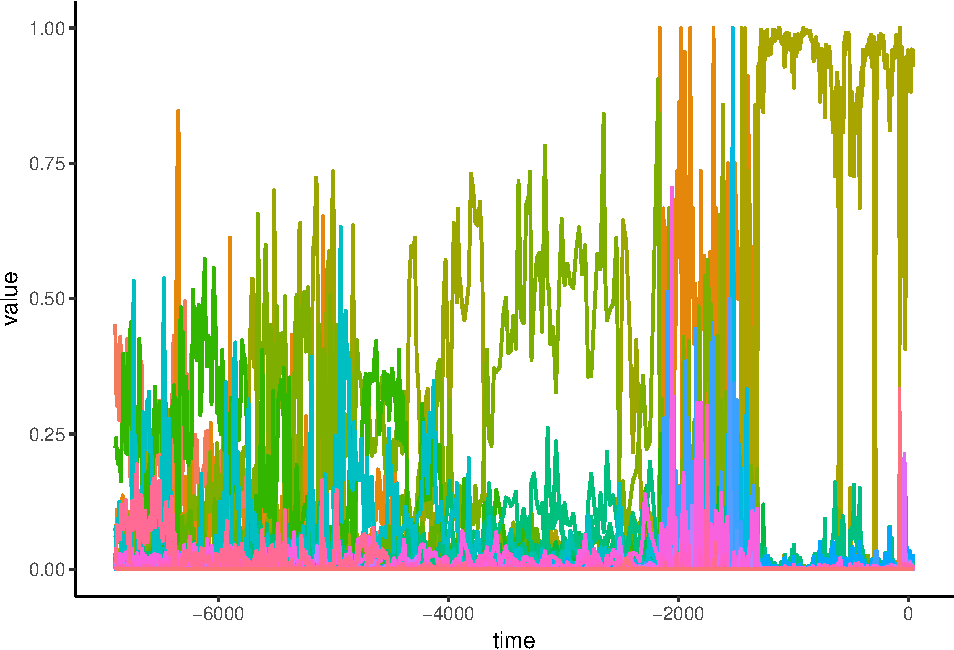
\includegraphics{myDissertation_files/figure-latex/unnamed-chunk-7-1.pdf}

\subsection{Plot the distance
travelled}\label{plot-the-distance-travelled}

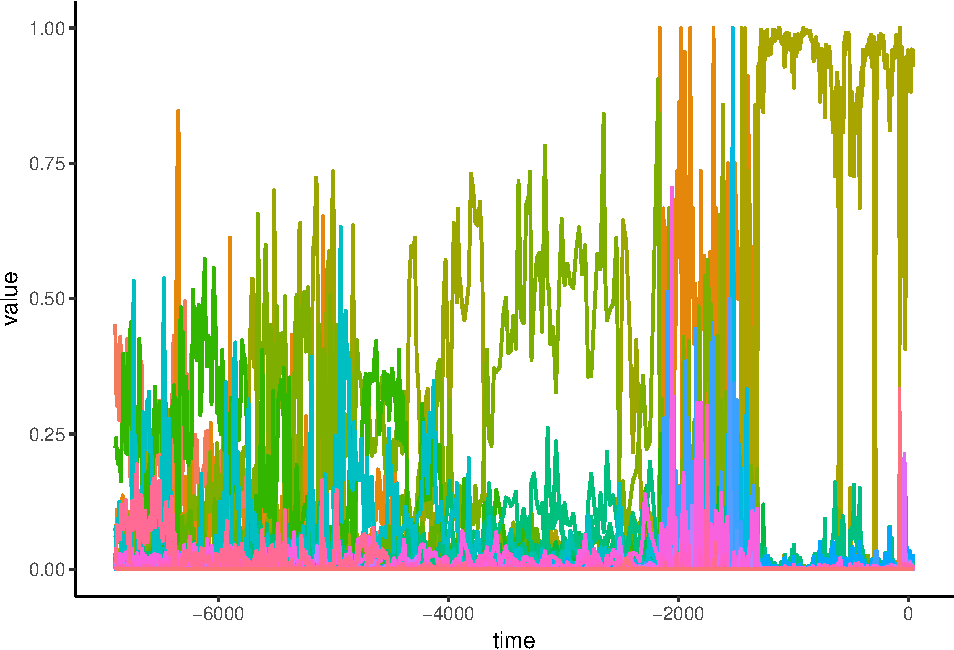
\includegraphics{myDissertation_files/figure-latex/unnamed-chunk-8-1.pdf}

\subsection{Plot the velocity}\label{plot-the-velocity}

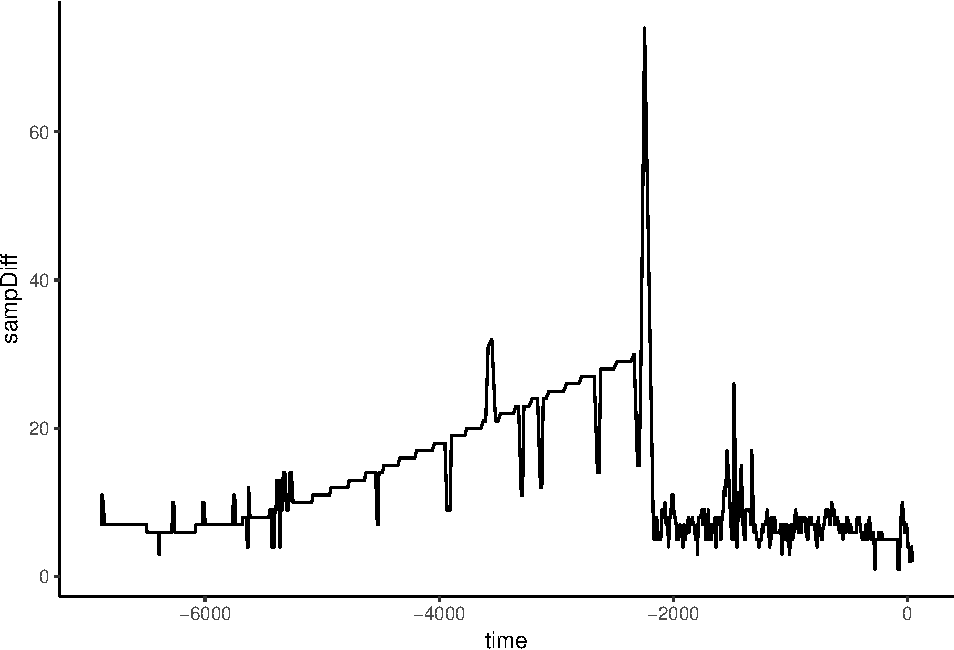
\includegraphics{myDissertation_files/figure-latex/unnamed-chunk-9-1.pdf}

\subsection{Plot the acceleration}\label{plot-the-acceleration}

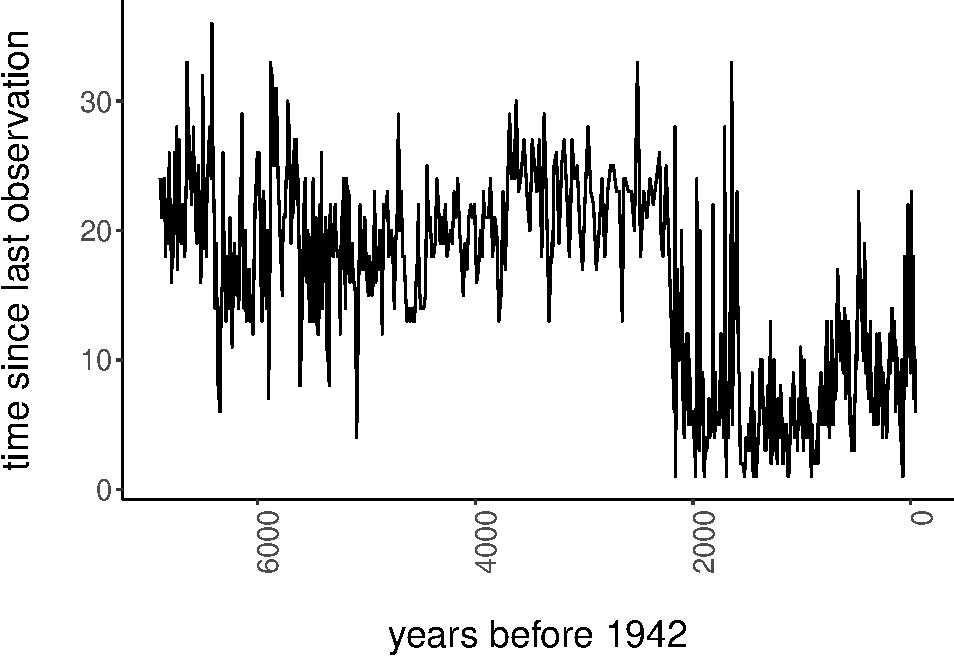
\includegraphics{myDissertation_files/figure-latex/unnamed-chunk-10-1.pdf}

\subsection{Plot a histogram of distance
traveled}\label{plot-a-histogram-of-distance-traveled}

Compare histogram of distance travelled to pdf calculated from velocity.

\includegraphics{myDissertation_files/figure-latex/unnamed-chunk-11-1.pdf}

\section{Moving window analysis}\label{moving-window-analysis}

\subsection{Specifcy parameters for the moving
window}\label{specifcy-parameters-for-the-moving-window}

Distance over which to move the window (in units time)
\begin{Shaded}
\begin{Highlighting}[]
\CommentTok{# Distance over which to move the window (in units time)}
\NormalTok{winspace <-}\StringTok{ }\DecValTok{50}

\CommentTok{# Size of the window (in units time)}
\NormalTok{winsize <-}\StringTok{ }\DecValTok{500}

\CommentTok{# Start and stop points for windows}
\NormalTok{t <-}\StringTok{ }\NormalTok{distance}\OperatorTok{$}\NormalTok{YB1950}
\NormalTok{winStart <-}\StringTok{ }\KeywordTok{seq}\NormalTok{(}\KeywordTok{min}\NormalTok{(t), }\KeywordTok{max}\NormalTok{(t), }\DataTypeTok{by =}\NormalTok{ winspace)}
\NormalTok{winStop <-}\StringTok{ }\NormalTok{winStart }\OperatorTok{+}\StringTok{ }\NormalTok{winsize}

\CommentTok{# Number of windows}
\NormalTok{nWin <-}\StringTok{ }\KeywordTok{length}\NormalTok{(winStart)}
\end{Highlighting}
\end{Shaded}
\subsection{Loop over data calculating a FI value for each
window}\label{loop-over-data-calculating-a-fi-value-for-each-window}

\section{Plots}\label{plots}

\subsection{Plot Fisher Information for each
window}\label{plot-fisher-information-for-each-window}

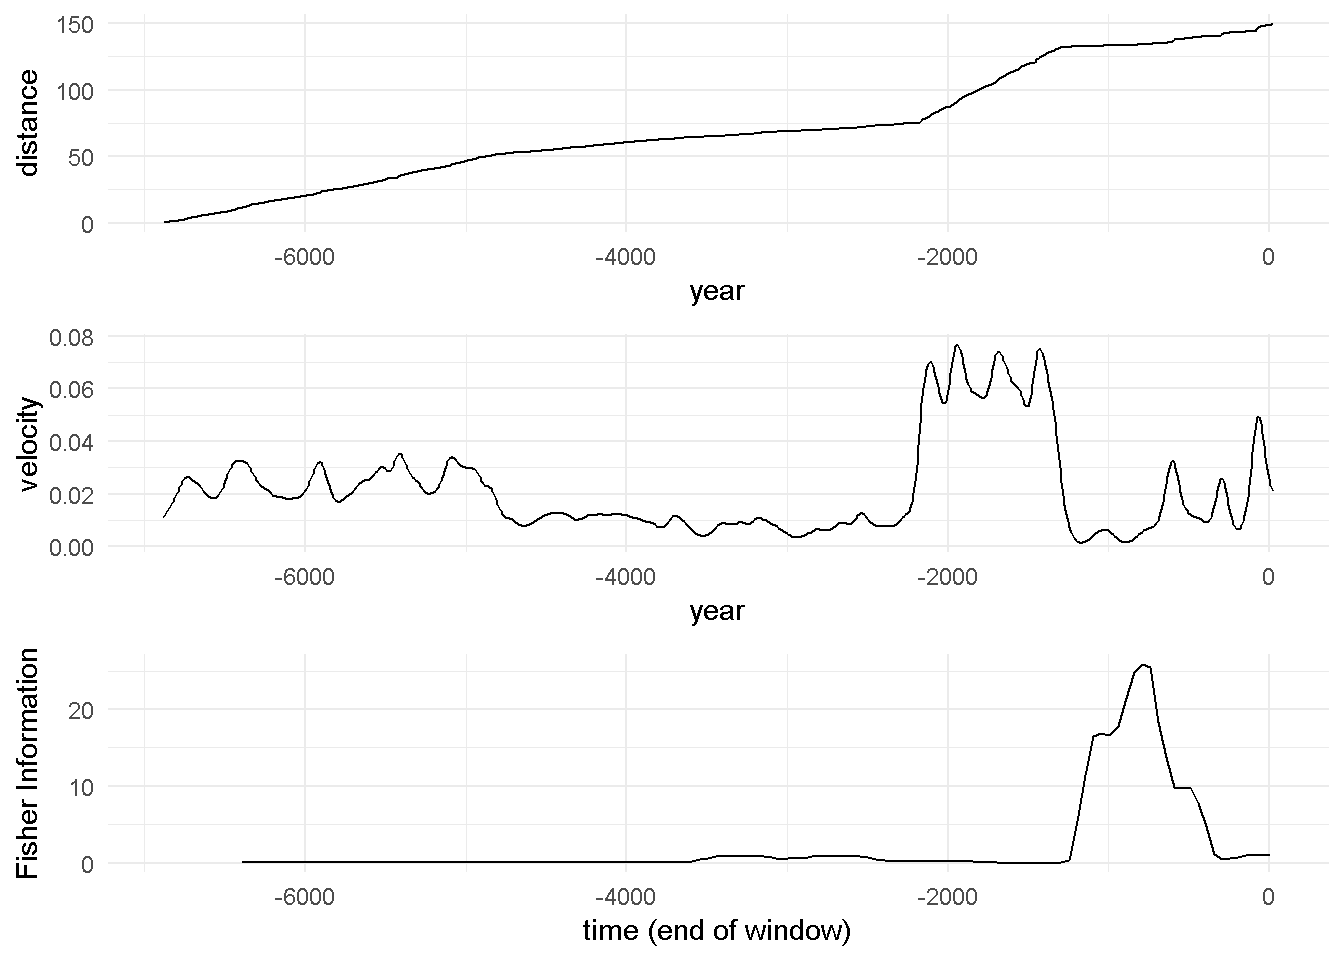
\includegraphics{myDissertation_files/figure-latex/FIplot-1.pdf}
\includegraphics{myDissertation_files/figure-latex/FIplot-2.pdf}

\subsection{Export figures}\label{export-figures}

\chapter*{Appendix B}\label{rRDM}
\addcontentsline{toc}{chapter}{Appendix B}

This appendix contains the vignette associated with the R Package,
\texttt{rRDM}. Development source code for this package is available on
GitHub as a compressed file,
\url{https://github.com/TrashBirdEcology/rRDM/archive/master.zip} or
\url{https://github.com/TrashBirdEcology/rRDM}.

\backmatter

\chapter*{References}\label{references}
\addcontentsline{toc}{chapter}{References}

\markboth{References}{References}

\noindent

\setlength{\parindent}{-0.20in} \setlength{\leftskip}{0.20in}
\setlength{\parskip}{8pt}

\hypertarget{refs}{}
\hypertarget{ref-abadi2010assessment}{}
Abadi, F., Gimenez, O., Arlettaz, R., \& Schaub, M. (2010). An
assessment of integrated population models: Bias, accuracy, and
violation of the assumption of independence. \emph{Ecology},
\emph{91}(1), 7--14.

\hypertarget{ref-andersen_ecological_2009}{}
Andersen, T., Carstensen, J., Hernández-García, E., \& Duarte, C. M.
(2009). Ecological thresholds and regime shifts: Approaches to
identification. \emph{Trends in Ecology \& Evolution}, \emph{24}(1),
49--57. \url{http://doi.org/10.1016/j.tree.2008.07.014}

\hypertarget{ref-angel2000}{}
Angel, E. (2000). \emph{Interactive computer graphics : A top-down
approach with opengl}. Boston, MA: Addison Wesley Longman.

\hypertarget{ref-angel2001}{}
Angel, E. (2001a). \emph{Batch-file computer graphics : A bottom-up
approach with quicktime}. Boston, MA: Wesley Addison Longman.

\hypertarget{ref-angel2002a}{}
Angel, E. (2001b). \emph{Test second book by angel}. Boston, MA: Wesley
Addison Longman.

\hypertarget{ref-beaugrand2004north}{}
Beaugrand, G. (2004). The north sea regime shift: Evidence, causes,
mechanisms and consequences. \emph{Progress in Oceanography},
\emph{60}(2-4), 245--262.

\hypertarget{ref-boettiger_quantifying_2012}{}
Boettiger, C., \& Hastings, A. (2012). Quantifying limits to detection
of early warning for critical transitions. \emph{Journal of the Royal
Society Interface}, \emph{9}, 2527--39.

\hypertarget{ref-cabezas_towards_2002}{}
Cabezas, H., \& Fath, B. D. (2002). Towards a theory of sustainable
systems. \emph{Fluid Phase Equilibria}, \emph{194}(Supplement C), 3--14.
\url{http://doi.org/10.1016/S0378-3812(01)00677-X}

\hypertarget{ref-cabezas_simulated_2005}{}
Cabezas, H., Pawlowski, C. W., Mayer, A. L., \& Hoagland, N. T. (2005).
Simulated experiments with complex sustainable systems: Ecology and
technology. \emph{Resources, Conservation and Recycling}, \emph{44}(3),
279--291. Retrieved from
\url{http://www.sciencedirect.com/science/article/pii/S092134490500025X}

\hypertarget{ref-chartrand_numerical_2011}{}
Chartrand, R. (2011). Numerical Differentiation of Noisy, Nonsmooth
Data. \emph{International Scholarly Research Notices}. Research article.
\url{http://doi.org/10.5402/2011/164564}

\hypertarget{ref-dakos_methods_2012}{}
Dakos, V., Carpenter, S. R., Brock, W. A., Ellison, A. M., Guttal, V.,
Ives, A. R., \ldots{} Nes, E. H. van. (2012). Methods for detecting
early warnings of critical transitions in time series illustrated using
simulated ecological data. \emph{PloS One}, \emph{7}(7), e41010.

\hypertarget{ref-fath_exergy_2004}{}
Fath, B. D., \& Cabezas, H. (2004). Exergy and Fisher Information as
ecological indices. \emph{Ecological Modelling}, \emph{174}(1), 25--35.
\url{http://doi.org/10.1016/j.ecolmodel.2003.12.045}

\hypertarget{ref-fath_regime_2003}{}
Fath, B. D., Cabezas, H., \& Pawlowski, C. W. (2003). Regime changes in
ecological systems: An information theory approach. \emph{Journal of
Theoretical Biology}, \emph{222}(4), 517--530.
\url{http://doi.org/10.1016/S0022-5193(03)00067-5}

\hypertarget{ref-fisher_mathematical_1922}{}
Fisher, R. A. (1922). On the Mathematical Foundations of Theoretical
Statistics. \emph{Philosophical Transactions of the Royal Society of
London. Series A, Containing Papers of a Mathematical or Physical
Character}, \emph{222}, 309--368. Retrieved from
\url{http://www.jstor.org/stable/91208}

\hypertarget{ref-frieden_physics_1998}{}
Frieden, B. R. (1998). \emph{Physics from Fisher information: A
unification.} New York, NY: Cambridge University Press.

\hypertarget{ref-frieden_exploratory_2007}{}
Frieden, B. R., \& Gatenby, R. (Eds.). (2007). \emph{Exploratory Data
Analysis Using Fisher Information}. Springer. Retrieved from
\url{http://www.springer.com/us/book/9781846285066}

\hypertarget{ref-hastings_regime_2010}{}
Hastings, A., \& Wysham, D. B. (2010). Regime shifts in ecological
systems can occur with no warning. \emph{Ecology Letters}, \emph{13}(4),
464--472. \url{http://doi.org/10.1111/j.1461-0248.2010.01439.x}

\hypertarget{ref-hefley2013statistical}{}
Hefley, T. J., Tyre, A. J., \& Blankenship, E. E. (2013). Statistical
indicators and state--space population models predict extinction in a
population of bobwhite quail. \emph{Theoretical Ecology}, \emph{6}(3),
319--331.

\hypertarget{ref-jorgensen_towards_2004}{}
Jorgensen, S. E., \& Svirezhev, Y. M. (2004). \emph{Towards a
Thermodynamic Theory for Ecological Systems}. Elsevier.

\hypertarget{ref-karunanithi_detection_2008}{}
Karunanithi, A. T., Cabezas, H., Frieden, B. R., \& Pawlowski, C. W.
(2008). Detection and assessment of ecosystem regime shifts from fisher
information. \emph{Ecology and Society}, \emph{13}(1).

\hypertarget{ref-mantua_methods_2004}{}
Mantua, N. (2004). Methods for detecting regime shifts in large marine
ecosystems: A review with approaches applied to North Pacific data.
\emph{Progress in Oceanography}, \emph{60}(2), 165--182.
\url{http://doi.org/10.1016/j.pocean.2004.02.016}

\hypertarget{ref-mayer_applications_2007}{}
Mayer, D. A. L., Pawlowski, D. C., Fath, P. B. D., \& Cabezas, D. H.
(2007). Applications of Fisher Information to the Management of
Sustainable Environmental Systems. In B. R. F. B. MS \& R. A. G. B. MD
(Eds.), \emph{Exploratory Data Analysis Using Fisher Information} (pp.
217--244). Springer London.
\url{http://doi.org/10.1007/978-1-84628-777-0_7}

\hypertarget{ref-perretti_model-free_2013}{}
Perretti, C. T., Munch, S. B., \& Sugihara, G. (2013). Model-free
forecasting outperforms the correct mechanistic model for simulated and
experimental data. \emph{Proceedings of the National Academy of
Sciences}, \emph{110}(13), 5253--5257.

\hypertarget{ref-petersen2008regime}{}
Petersen, J. K., Hansen, J. W., Laursen, M. B., Clausen, P., Carstensen,
J., \& Conley, D. J. (2008). Regime shift in a coastal marine ecosystem.
\emph{Ecological Applications}, \emph{18}(2), 497--510.

\hypertarget{ref-rodionov_application_2005}{}
Rodionov, S., \& Overland, J. E. (2005). Application of a sequential
regime shift detection method to the Bering Sea ecosystem. \emph{ICES
Journal of Marine Science}, \emph{62}(3), 328--332.
\url{http://doi.org/10.1016/j.icesjms.2005.01.013}

\hypertarget{ref-roy_frieden_physics_1998}{}
Roy Frieden, B. (1998). \emph{Physics from Fisher information}.
Cambridge: Cambridge University Press.

\hypertarget{ref-scheffer_catastrophic_2001}{}
Scheffer, M., Carpenter, S., Foley, J. A., Folke, C., \& Walker, B.
(2001). Catastrophic shifts in ecosystems. \emph{Nature},
\emph{413}(6856), 591--596.

\hypertarget{ref-spanbauer_prolonged_2014}{}
Spanbauer, T. L., Allen, C. R., Angeler, D. G., Eason, T., Fritz, S. C.,
Garmestani, A. S., \ldots{} Stone, J. R. (2014). Prolonged instability
prior to a regime shift. \emph{PLoS One}, \emph{9}(10), e108936.


% Index?

\end{document}
